\documentclass[12pt,a4paper,twoside,final]{report}
%
%\usepackage{ngerman}            %Neue Rechtschreibung
\usepackage{graphicx}           %Graphiken einbinden
\usepackage[export]{adjustbox}	%Adding frames to graphics
\usepackage{subcaption}
\usepackage{fontenc}            %Verwenden von \"{o} \"{a} \"{u} {\ss}
\usepackage[latin1]{inputenc}   %Verwenden von \"{o} \"{a} \"{u} {\ss}
\usepackage{fancyhdr}           %Kopf-und Fusszeilen
\usepackage{theorem}
\usepackage{amsmath}
\usepackage{amssymb}
\usepackage{natbib}
\usepackage{parskip}
\usepackage{longtable}
\usepackage{helvet}
\usepackage[right]{eurosym}
\usepackage{pdflscape}
\usepackage[compact]{titlesec}
\usepackage{siunitx}
\usepackage{booktabs}
\usepackage{setspace}
\usepackage{tikz}
\usetikzlibrary{positioning}
\usetikzlibrary{calc}
\usetikzlibrary{shapes.geometric}
\usetikzlibrary{shapes.arrows}
\usetikzlibrary{decorations}
\usetikzlibrary{decorations.pathmorphing}
\usetikzlibrary{decorations.text}
\usetikzlibrary{decorations.markings}
\usetikzlibrary{backgrounds}
\usetikzlibrary{intersections}
\usepackage{grffile}
\usepackage{zref-xr}

\usepackage[a4paper,
			textwidth = 16.5cm,
			textheight = 25cm,
			inner = 2.5cm]{geometry}
		
		
\usepackage[pdftex,
			colorlinks,
			linkcolor = black,
			citecolor = black]{hyperref}
%
%--------------------------------------------------------------------
%
%Kopf- und Fu�zeile
%
\pagestyle{fancyplain}
 \renewcommand{\chaptermark}[1]{\markboth{#1}{}}
 \renewcommand{\sectionmark}[1]{\markright{\thesection\ #1}}
 \lhead[\fancyplain{}{\sl\thepage}]{\fancyplain{}{\sl\rightmark}}
 \rhead[\fancyplain{}{\sl\leftmark}]{\fancyplain{}{\sl\thepage}}
 \lfoot{}
 \cfoot{}
 \rfoot{}
%--------------------------------------------------------------------
%
%Definition der Abschnitts�berschriften
%
\titleformat{\chapter}[hang]{\normalfont\huge\bfseries}{\thechapter}{16pt}{\huge}{}
%\renewcommand{\thesection}{\alph{section}}
\titleformat{\section}[hang]{\Large\bfseries}{\thesection}{10pt}{}
%
%--------------------------------------------------------------------
%
%Kommandos f�r die Titelseitendaten
%
\newcommand{\VersuchNummer}[1]{\newcommand{\VNummer}{#1}}
\newcommand{\VersuchName}[1]{\newcommand{\VName}{#1}}
\newcommand{\Studiensemester}[1]{\newcommand{\SSemester}{#1}}
\newcommand{\VersuchDatum}[1]{\newcommand{\VDatum}{#1}}
\newcommand{\Bearbeiter}[1]{\newcommand{\VBearbeiter}{#1}}
%
%--------------------------------------------------------------------
%
\newcounter{requirementcount}
\setcounter{requirementcount}{1}
%
%Titelseite
%
%Daten zum Versuchsprotokoll f�r das Praktikum Elektrische Antriebe
%
%Eingegeben werden:
%
% - Die Nummer und Name des Versuchs:
%     1 Asynchronmaschine
%     2 Gleichstrommaschine
%     3 B�rstenloser Gleichstrommotor
%     4 Schrittmotor
%
\VersuchNummer{1}
\VersuchName{Asynchronmaschine}
%
%------
%
%------
%
% - Studiensemester des Bearbeiters
\Studiensemester{6}
%
%------
%
% - Datum der Versuchsdurchf�hrung
%
\VersuchDatum{22.11.2018}
%
%------
%
% - Namen der Bearbeiter in der Gruppe
%
\Bearbeiter{Max Antriebslos, Johann Ohneland, Hans Lackland}
%
\renewcommand\maketitle{
\begin{titlepage}

\thispagestyle{empty}
%
\begin{tabular}[t]{lp{0.25\textwidth}r}
%

\includegraphics[width = 0.25\textwidth]{./Bilder/Logo_HSRT_TEC_RGB.png}
%
&&
\includegraphics[width = 0.4\textwidth]{./Bilder/Logo_HSRT_Schwarz.jpg}
%
\end{tabular}
%

\renewcommand{\baselinestretch}{1.2}

\sf\large\textbf{Hochschule Reutlingen}\\
\sf\large\textbf{Fakult�t Technik}\\

\vspace{7cm}

{\sf\Huge\textbf{Bachelor thesis}}\\
%
\vspace{0.5cm}

{\sf\huge{Sensor-based navigation of a robot under ROS with triangulation scanner}}\\


\vspace{4.5cm}

\renewcommand{\arraystretch}{2}
%\begin{tabular}{|p{0.33\textwidth}p{0.33\textwidth}p{0.33\textwidth}|}
%%
%\hline
%\multicolumn{2}{|p{0.66\textwidth}|}{Datum:~\VDatum}				&Studiensemester:~\SSemester		\\
%\hline
%\multicolumn{3}{|l|}{\VBearbeiter}\\
%\hline
%%
%\end{tabular}
\renewcommand{\arraystretch}{1}

\renewcommand{\baselinestretch}{1}
%

\vfill
%


\includegraphics[width = \textwidth]{./Bilder/Silhouette_HSRT_045K.jpg}
%
\newpage
\ 
\thispagestyle{empty}
%
\end{titlepage}}
%
%--------------------------------------------------------------------
%
\begin{document}
%


\maketitle
\setcounter{page}{1}
\spacing{1.5}

%
%
%       In diesem Dokument werden die Aufgaben als Einzeldateien eingebunden.
%       Jede Aufgabe wird in einer eigenen Datei eingetragen
%       Dies ist unten stehend anhand der Dateien aufgabe1.tex und aufgabe2.tex dargestellt.
%
%       Prinzipiell k�nnte der gesamte Code auch direkt eingebunden werden. 
%       Dies ist jedoch weniger �bersichtlich
%
%
%---------------------------------------------------------------------
%

%--------------------------------------------------------------------
%
%Mustervorlage fuer eine Aufgabe
%
%--------------------------------------------------------------------
%
%Ueberschreiben der automatisch erzeugten Aufgabennummer
%Die folgende Aufgabennummer ergibt sich aus dem Stand des
%Z�hlers + 1
%\setcounter{chapter}{0}
%
% 2 pages
\chapter{Introduction}\label{chap:introduction}
%
%Teilaufgabe 1

%
\section{Motivation}\label{sec:motivation}
%
Mobile robots have received much attention in the past few years. The number of applications of mobile robots, especially in the industry, has increased enormously. The autonomous navigation is one of the main challenges in the design and implementation of mobile robots. The approaches developed for the navigation of mobile robots are very diverse. Most of these approaches are based on several hardware components, such as embedded laser scanners, odometry sensors, and other components. Thus, developing an approach where only one sensor is used instead of several sensors will decrease the robot's costs.\\
Furthermore, the development of mobile is a complex process. The motivation behind this project is to develop a maintainable robot navigation approach that can be transferable and adaptable to other robots and hardware components.  This can be done by using ROS, which will be explained in later chapters.
%
%---------------------------------------------------------------------
%
\section{Problem Statement}\label{sec:problemStatement}
%
This project is divided into several hardware and software components. The main element is the PC, which can be seen as a master. Other elements, such as a triangulation laser scanner, a lego boost robot, localization algorithms, and motion control algorithms can be viewed as slaves.\\
First, a ROS system must be installed and created on the PC. Then a simple Lego Boost robot must be assembled, including the robot's connection to the PC. A triangulation laser scanner must be later integrated into the system. The next problem is the implementation of the localization algorithms. Lastly, the motion control algorithms must be implemented and integrated into the system. 
%
%---------------------------------------------------------------------
%
\section{Aim}\label{sec:aim}
%
The final aim of this project is to build a ROS system consisting of a Lego Boost robot, a triangulation sensor, a localization and control algorithm. All these components are represented by individual ROS nodes. The triangulation sensor is fixed in the room, and the controller lets the robot follow a user-predefined path in the room.
%--------------------------------------------------------------------
%
%Mustervorlage fuer eine Aufgabe
%
%--------------------------------------------------------------------
%
%Ueberschreiben der automatisch erzeugten Aufgabennummer
%Die folgende Aufgabennummer ergibt sich aus dem Stand des
%Z�hlers + 1
%\setcounter{chapter}{0}
%
%
% 10 pages
\chapter{Theoretical Background}\label{chap:literatureReview}
%
The core of the field of mechatronics is the combination of both hardware and software. A fundamental aspect in the field of mechatronics is the modularisation. Modularisation takes place both on the hardware and on the software level. The hardware modules used in this project are a differential driver robot and a triangulation laser scanner. On the other side, ROS is responsible for the implementation of the software modules.  
Before going deep into the implementation of the project and the methods used to solve the problem,  both software and hardware modules will be explained.
%
%Teilaufgabe 1
%
\section{Robots Operating System ROS}\label{sec:ros}
%3 pages
Designing robots in general, especially mobile robots, is considered as one of the essential elements of the industrial revolutions over the past decades.  However, designing a robot is a complicated procedure. The main reason for that complicity is that robots' platforms consist of two main components, namely the hardware and the software applications. 

The hardware of robots could be, i.e., sensors, motors, and actuators. On the other hand, software applications are responsible for doing a specific functionality, such as navigation, localization, or object recognition \cite{calis_roboter_2020}.


\subsection{Robot Software Platforms}
In order to simplify the robots' design procedure, scientists and researches were trying to develop so-called "Robot Software Platforms."  In the literature, there seems to be no specific definition of Robot Software Platforms. However, robots software platforms can be interpreted as a middleware between the hardware components and the software modules, allowing developers to design seperated software modules, that could run on different hardware components without reprogramming the developed software module according to the different low-level drivers of each component \cite{joseph_learning_2018}\cite{yoonseok_ros_2017} \cite{calis_roboter_2020}. For example, a software module could be developed for navigation. By integrating this module in a robot software platform, it can run on different robots without dealing with each robot's underlying complexity. Using a proper robot software platform depends on each robot's purpose and requirements, as each platform has its advantages and disadvantages. One of the most used robot software platforms is ROS. ROS stands for Robot Operating System, which is confusing, since ROS is not an operating system by itself. Instead, it runs on an operating system like Linux and can be seen as a layer between an operating system and robot's applications, as shown in figure \ref{fig2_1} \cite{yoonseok_ros_2017}.
\begin{figure}[ht]
	\centering
	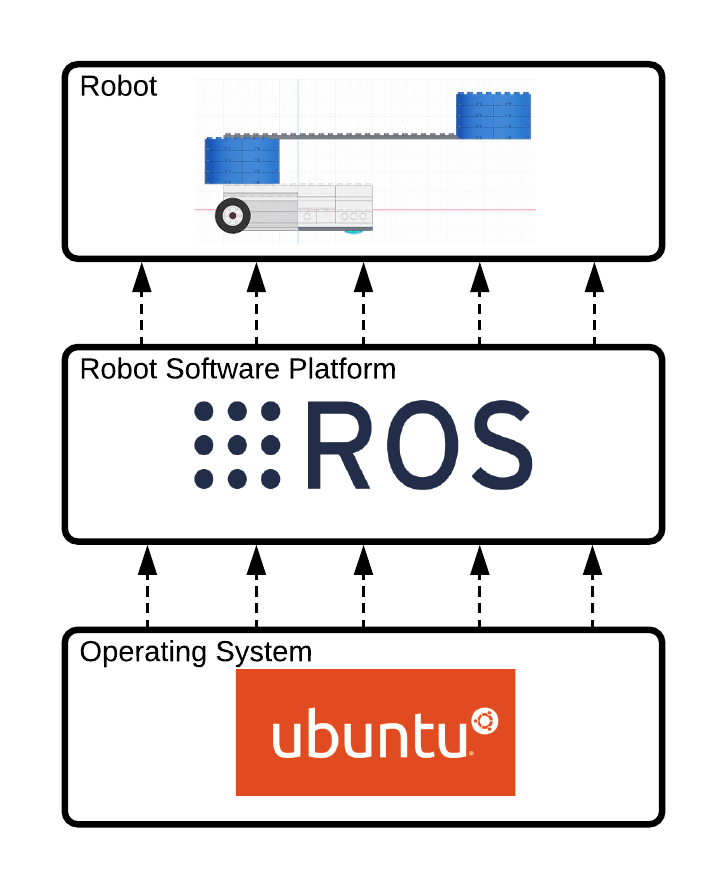
\includegraphics[width = 0.6 \textwidth, frame]{./Bilder/roslayers.png}			\caption{ROS as middleware between robots and operating systems}
	\label{fig2_1}
\end{figure}

ROS has been chosen over other platforms for the implementation of the application developed in this thesis because of its ecosystem and the enormous amount of packages that are ready to be used and integrated into the application. Another advantage of ROS is its simplicity to learn. One of the ROS disadvantages is that it is not a real-time robot software platform, as it is built on Linux. However, realtime applications can be developed on ROS2, which is the next version of ROS.
ROS versions are always tied to Ubuntu LTS (Long Term Support) versions and are released simultaneously, namely every two years. The used version of ROS in this project is ROS Melodic, which runs on Ubuntu 18.04. The next version of ROS is ROS Neotic, which runs on Ubuntu 20.04. ROS Noetic would be the last version of ROS. After that, ROS2 will be used instead.  


\subsection{ROS Working Principle}
ROS working principle is explained in the literature in different ways. As explained in \cite{calis_roboter_2020}, ROS is based on a publish/subscribe concept, where processes communicate with each other via a message system. The best way to explain how ROS works is to analyze this publish/subscribe concept and explain the message system's main components and how messages are exchanged. This subsection explains the working principle of the ROS based on its description given in \cite{yoonseok_ros_2017}.

ROS applications consist of different processes, where each process is responsible for specific functionality such as navigation, path planning, or processing sensor data and so forth. These processes are called nodes. These nodes exchange information with each other in the form of messages. Each node can contain a publisher, that sends messages to a topic, or a subscriber, that receives messages from a topic, or both. A topic can be interpreted as a container that contains messages in nodes. TCPROS is the protocol that is responsible for exchanging the messages between different nodes in ROS, and it is based on a TCP/IP protocol. 
The central node in any ROS application is the master node, which is responsible for matching the information of the nodes with each other. In figure \ref{fig2_2}, the steps needed for establishing a communication between a publisher node and a subscriber node is displayed. First, the subscriber sends its information to the master node. This information contains, for example, the URI of the node, and the topics in the node. Next, the publisher sends its information to the master. The master then passes the publisher's information to the subscriber. The subscriber now recognizes the publisher, and the communication is established. The task of the master node is only to exchange the nodes' information. Once the nodes recognize each other, the master node role is completed.
ROS nodes also contain other information other than publishers and subscribers, such as parameters, service servers, and action servers. 
\begin{figure}[ht]
	\centering
	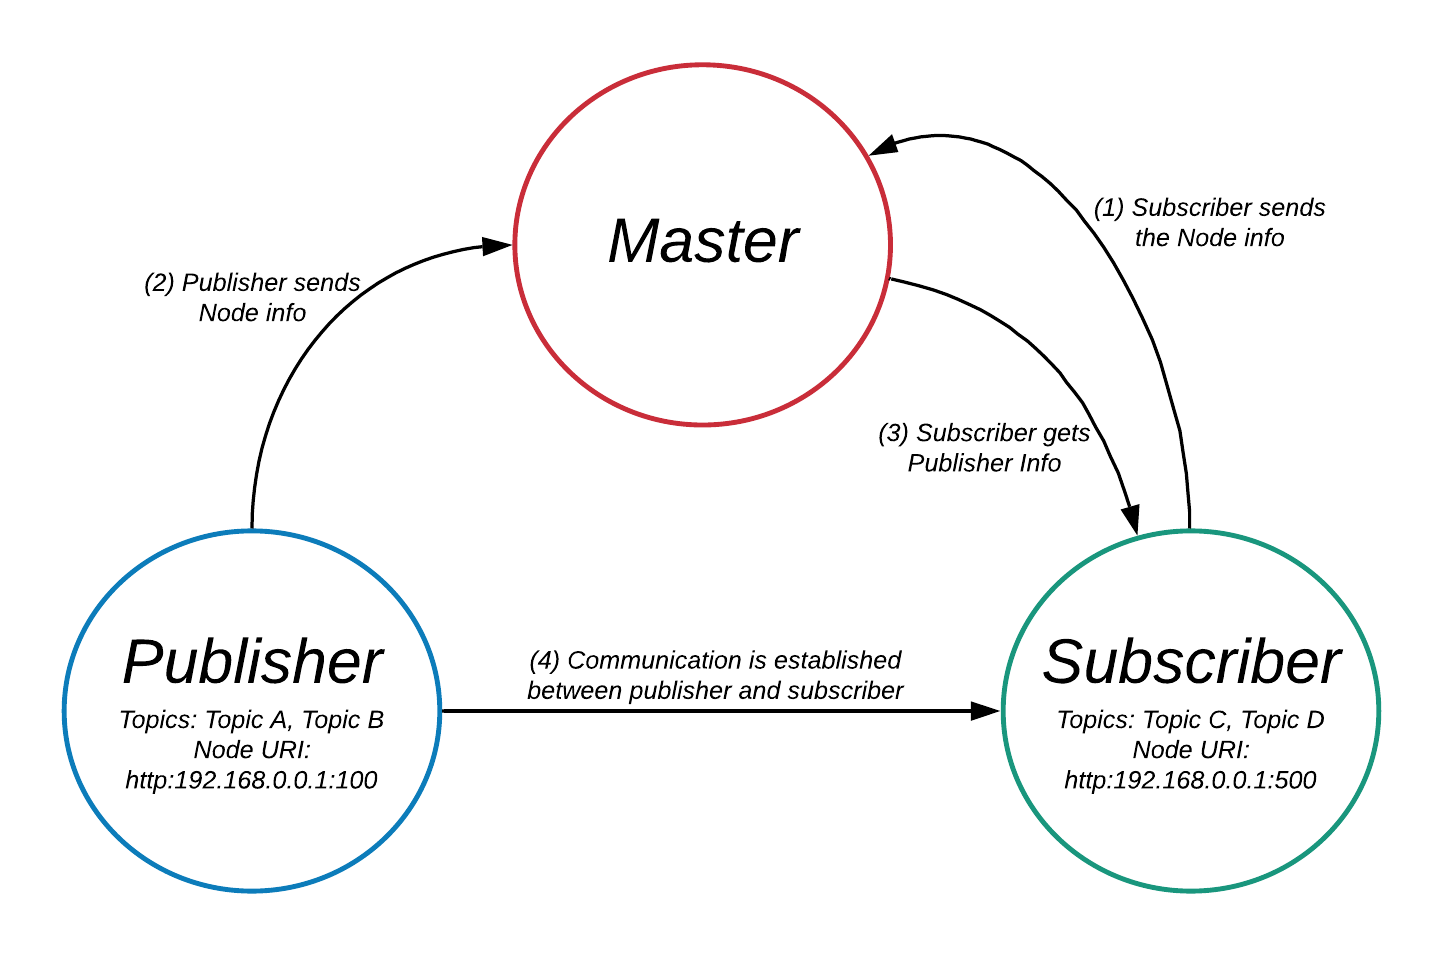
\includegraphics[width = 0.8\textwidth, frame]{./Bilder/umlROS.png}			\caption{ROS architecture design}
	\label{fig2_2}
\end{figure}


As described in \cite{noauthor_catkin_nodate}, ROS has its own build system, which is called catkin. In each ROS project, a file called "CMakeLists.txt" must be defined. This file contains the dependencies of the project that are needed for the build process. Catkin is also responsible for creating the workspace, in which all project components are installed. Inside the catkin workspace, the project packages are defined. Packages in ROS can be interpreted as libraries. Each package contains files, in which nodes, messages, services, and functionalities are defined.


In summary, it is important to know that ROS's core feature is the modularization in terms of software. Modularization has many advantages, such as code reuse and working on loosely coupled processes.  
%
%--------------------------------------------------------------------
%
%
\section{Differential Driver Robots}\label{sec:legoboost}
%3 pages

The definition of mobile robots is usually associated with autonomous movement. As explained in \cite{tzafestas_introduction_2013}, mobile robots are autonomously moving robots that can reach a specific goal. Therefore, an essential property of mobile robots is that they can plan their motion independently. Mobile robots are differentiated based on the environment they are used in, such as air, ground, and water \cite{rubio_review_2019}. Thus, the definition of mobile robots does not just include wheeled mobile robots, but generally, any robot that can move autonomously, such as drones, wheeled robots, or even legged robots. As shown in figure \ref{fig2_3}, wheeled mobile robots can be classified into three main categories: car-like mobile robots, omnidirectional mobile robots, and differential mobile robots \cite{tzafestas_introduction_2013}. 

\begin{figure}[ht]
\centering
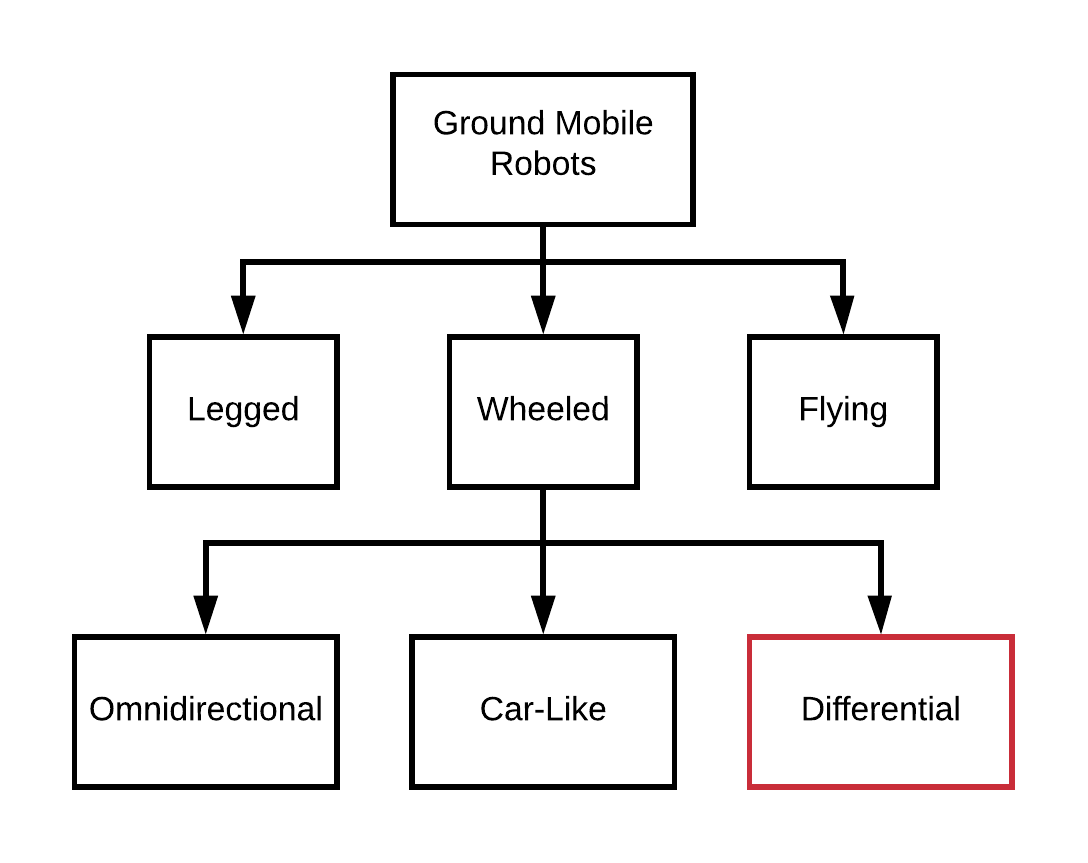
\includegraphics[width = 0.6\textwidth, frame]{./Bilder/robottypes.png}
\caption{Different types of ground mobile robots}
\label{fig2_3}
\end{figure}

The difference between these categories relies on the driving system of each robot. This subsection gives a theoretical explanation of the differential mobile robots since it is the type of mobile robot used for the project.

Differentially driven mobile robots are used in various applications, such as internal logistics or automated gastronomy, due to its design simplicity. As shown in figure \ref{fig2_4}, the drive system of differentially driven mobile robots consists of two wheels placed on the right and the left side of the robot, where each wheel is controlled by a separate motor \cite{tzafestas_introduction_2013}. Moreover, most of the time, there is one more omnidirectional wheel or a caster wheel that provides the stability of the robot. This wheel enables the robot to move even on uneven surfaces. The speed and direction of the right and left wheels determine the robot's motion. By using different wheel speeds and directions, the motion of differentially driven robots can be explained as an arc around a point, which is the Instantaneous Center of Rotation (ICR), as shown in figure \ref{fig2_4} \cite{corke_robotics_2017}. 
\begin{figure}[ht]
\centering
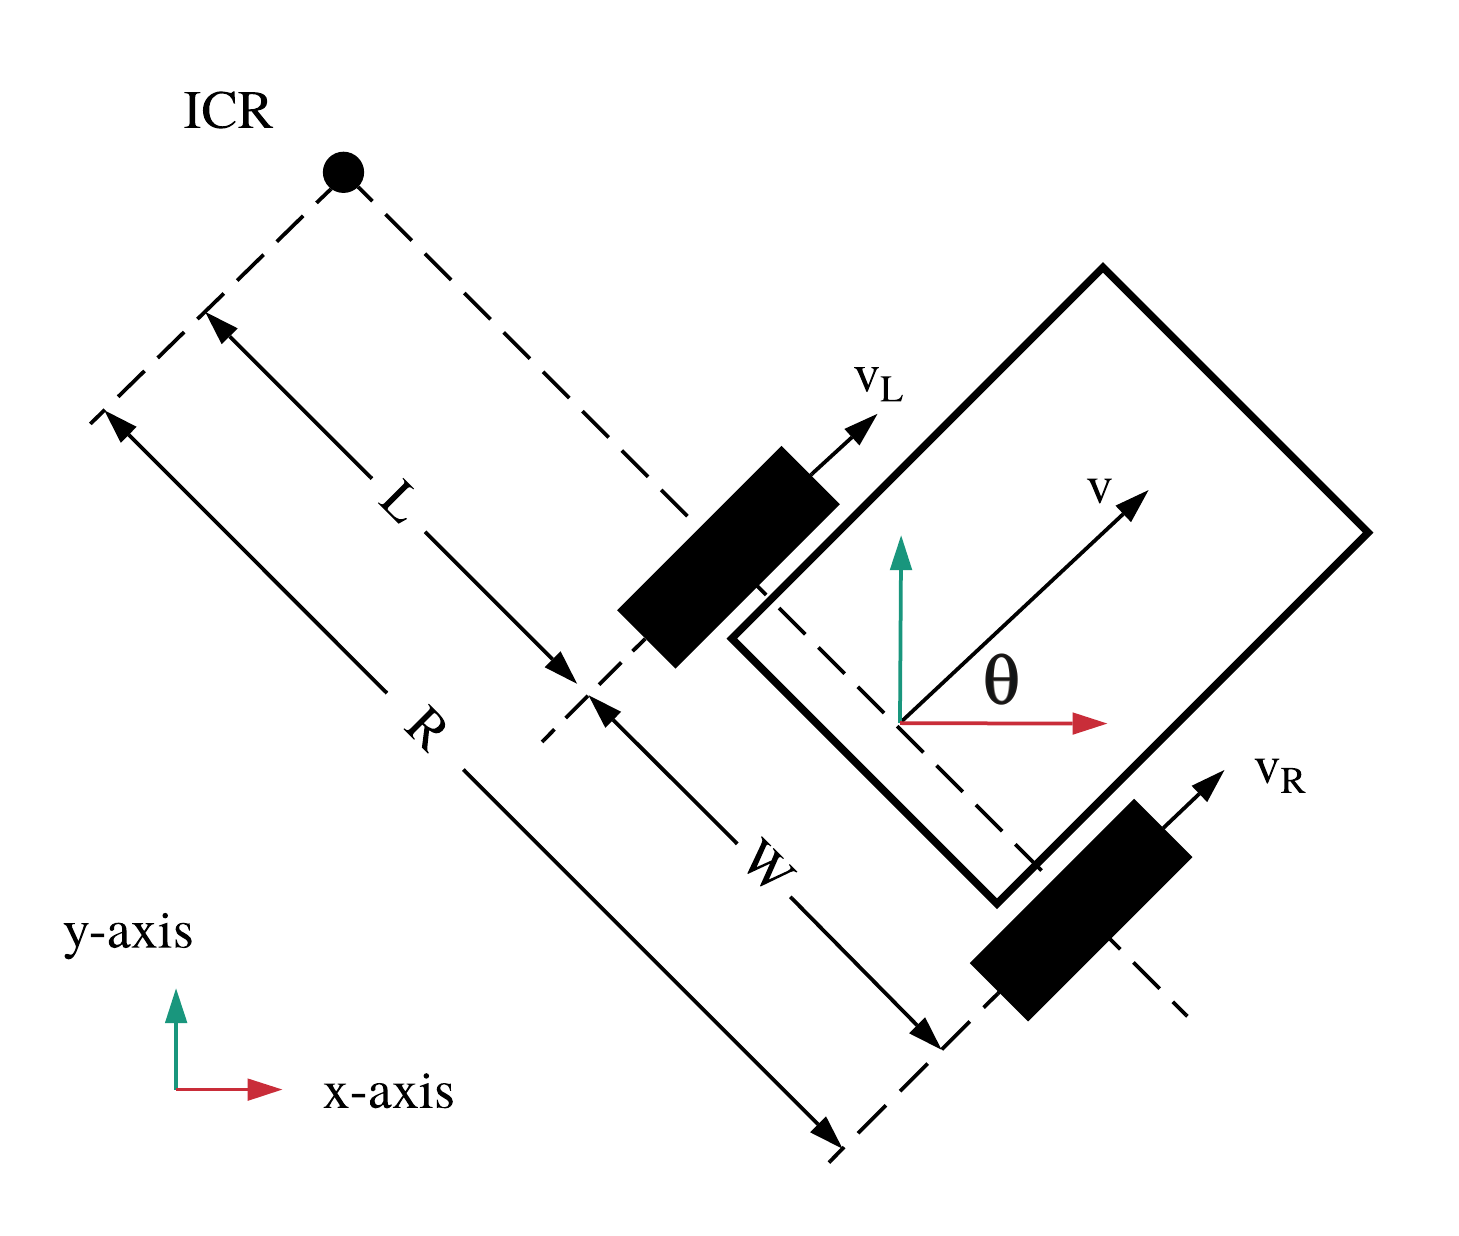
\includegraphics[width = 0.7\textwidth, frame]{./Bilder/differentialdrive.png}
\caption{Basic design of a differential driven mobile robot}
\label{fig2_4}
\end{figure}
The properties of the ICR, namely, the distance between the robot and the ICR, can be determined by knowing the velocity of each wheel and the distance between the wheels. This kinematic model is explained in \cite{corke_robotics_2017} as follows:

\begin{equation} \label{eq2_1}
\dot{\theta} = \frac{v_L}{L} = \frac{v_R}{R} 
\end{equation}
\begin{equation} \label{eq2_2}
\dot{\theta} = \frac{v_R-v_L}{W} 
\end{equation}
\begin{equation} \label{eq2_3}
\dot{x} = v \cdot cos(\theta)\\
\end{equation}
\begin{equation} \label{eq2_4}
\dot{y} = v \cdot sin(\theta)\\
\end{equation}
\begin{equation} \label{eq2_5}
\dot{\theta} =\frac{v_\Delta}{W}
\end{equation}
where \hspace{13mm} $v_L, v_R$ are the velocities of left and right wheels, respectively\\ 
	  \hspace*{25mm} $L, R$ are the distance from IPC to the left and right wheels, respectively\\
 	  \hspace*{25mm} $W$ is the distance between the left and right wheels\\
 	  \hspace*{25mm} $v_\Delta$ = $v_R-v_L$\\
 	  \hspace*{25mm} $v$ = $\frac{1}{2}\cdot(v_R+v_L)$\\
	  

By using these equations, a control algorithm can be designed to achieve a specific goal such as, following a trajectory, or following a line, or moving to a specific point. The implementation of the control algorithm is explained in a later chapter.
%
%
%--------------------------------------------------------------------
%
%

\section{Triangulation Laser Scanner}\label{sec:lidar}
%1 pages

Another module of the project is the laser scanner. The laser scanner is used to localize the differential driver robot position and orientation. The implementation of the localization process is discussed in later chapters. In this section, the advantage of the triangulation laser scanner compared to other types of sensors is discussed as well as the working principle of the specific sensor used.

\subsection{Localization Sensors and Methods}
\textbf{Wheel Odometry:}\\
The position of the robot can be estimated by using  rotary encoders. The rotary encoders are embedded in each wheel. The idea behind rotary encoders is to calculate the number of revolutions of the wheel.  By knowing the radius of the wheel, the moved distance can be then calculated. The wheel odometry method is simple and is used in many applications. However, several problems occur while implementing this method. As described in \cite{aqel_review_2016}, the main problem is the position draft due to the wheel slippage. This leads to inaccurate position estimation.

\textbf{GPS:}\\
Global Positioning System (GPS) is another localization method that can be used. It is used in different applications as transportations, agriculture, and aviation. Using a GPS receiver, the position of the robot can be determined with the help of four satellites. The main problem with using a GPS sensor is its measurement accuracy. For example, Adafruit Ultimate GPS has an accuracy of 3 meters and costs around 40\euro  \cite{industries_adafruit_nodate}. Another sensor is SparkFun GPS-RTK2, which has an accuracy of 2.5 meters and costs around 200 \euro \cite{noauthor_sparkfun_nodate}. Another problem is the reduction of accuracy in indoor applications. Thus, GPS sensor-based applications are used outdoors due to week signals from the GPS satellites.

\textbf{Ultrasonic Sensors:}\\
Ultrasonic sensors measure the distance to an obstacle by using ultrasonic waves. As described in \cite{aqel_review_2016}, the major disadvantage of ultrasonic sensors is the dependence on the material and the orientation of the measured object surface. Another disadvantage of the ultrasonic sensors is the poor lateral resolution (also called angular resolution). Additionally, the noise of the environment affects the accuracy of the measurement. In figure \ref{ultrasonic} is an example of ultrasonic sensors.

\begin{figure}[ht]
\centering
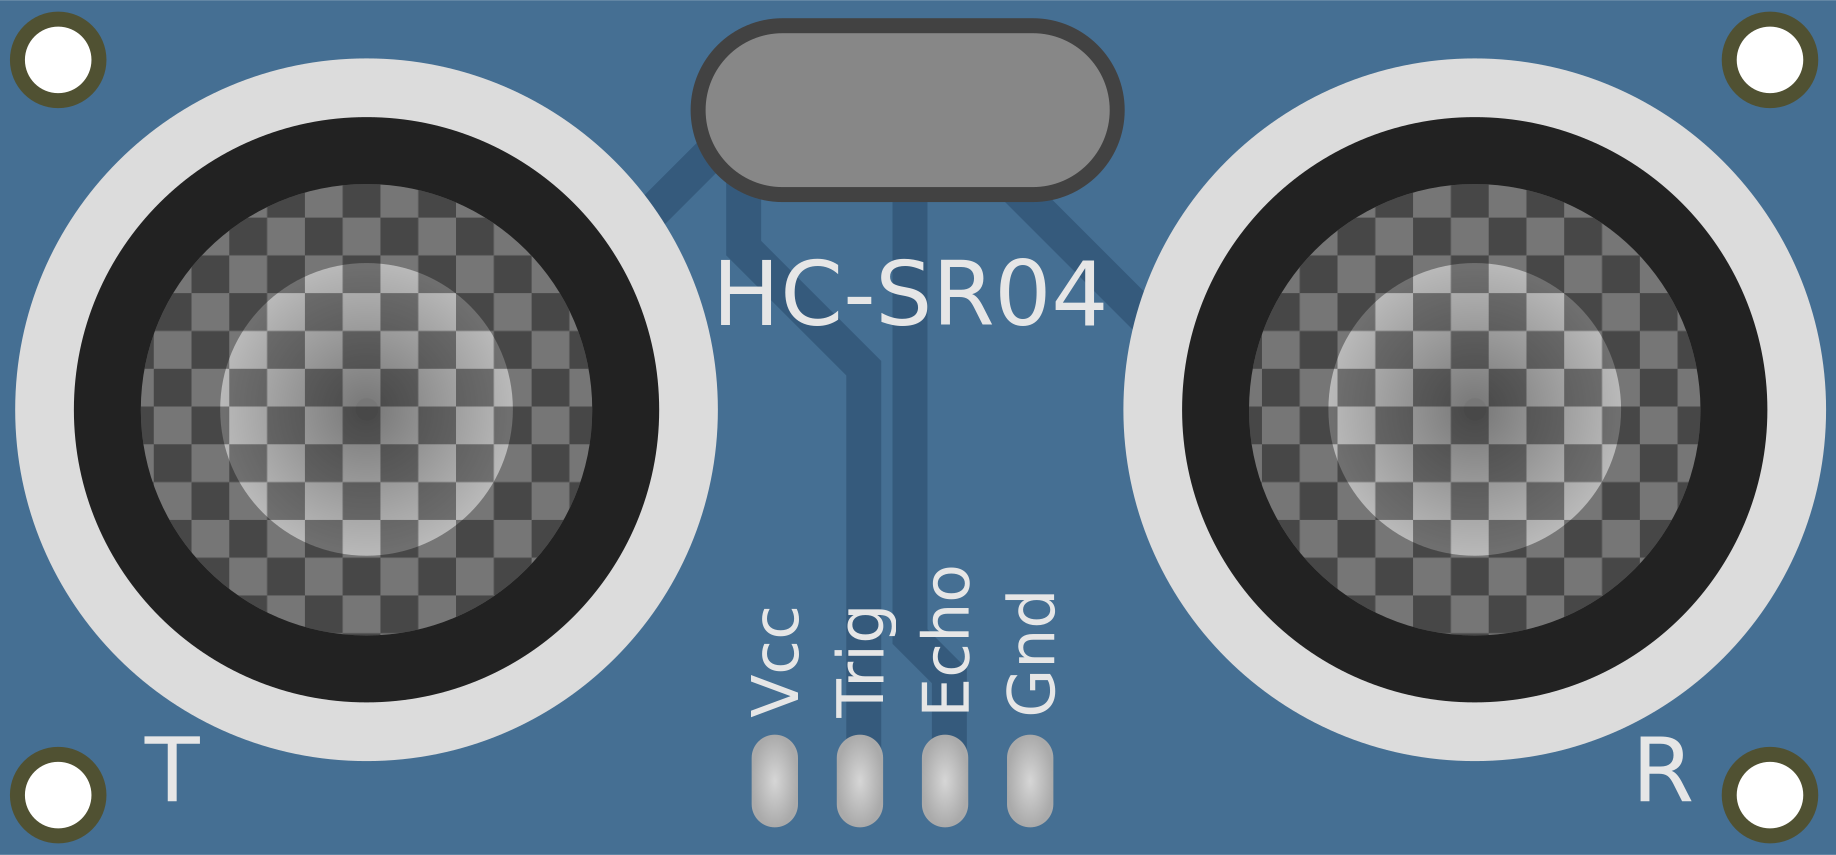
\includegraphics[width = 0.5\textwidth, frame]{./Bilder/Ultrasonic.png}
\caption{Ultrasonic sensor}
\label{ultrasonic}
\end{figure}

\textbf{Laser Sensors:}\\
Laser sensors are widely used for navigation and localization purposes. The application purpose of laser sensors is similar to ultrasonic sensors, where the distances to objects are detected. Laser sensors, however, as the name indicates, use a laser instead of ultrasonic waves. Laser sensors can be specified into two main types, namely position-based (triangulation) or time-based (LIDAR) sensors. LIDAR sensors calculate the distance to an object by measuring the time the laser took from the laser source to the object and back.  An example of LIDAR sensors is the Sick 2D-Laserscanner LMS100, which costs around 3000 \euro.

Triangulation Laser scanners use another technique to measure the distance to objects. It does not use the time of flight but the direction of the reflected light to determine the range of an object. In this project, the triangulation laser scanner YDLIDAR X2 which is displayed in figure \ref{ydlidar}, is used. It costs around 70 \euro, which is much cheaper than LIDAR sensors. The working principle of the triangulation laser scanner will be discussed in the following subsection. 

\begin{figure}[ht]
\centering
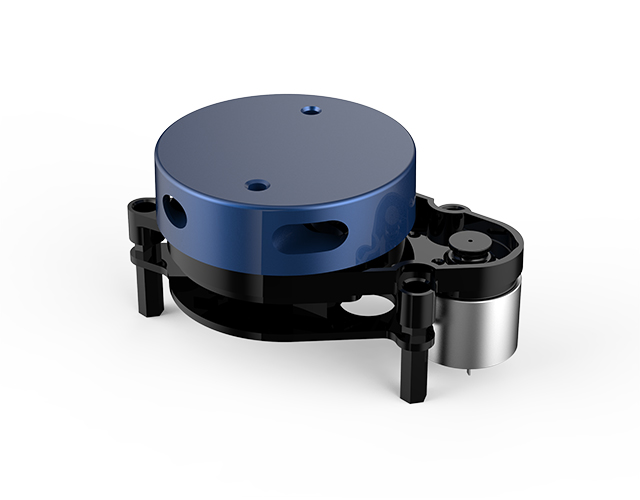
\includegraphics[width = 0.5\textwidth, frame]{./Bilder/ydlidar.jpg}
\caption{YDLIDAR X2 triangulation laser scanner. \textcopyright YDLIDAR All rights reserved }
\label{ydlidar}
\end{figure}

As explained in \cite{aqel_review_2016}, the following table describes the advantages and disadvantages of each sensor. 

\begin{table}[h]
\centering
\begin{tabular}{|| c | l | l ||} 
 \hline
 Sensor  & Advantages & Disadvantage \\ [0.5ex] 
 \hline\hline
 Wheel Odometry & \makecell[l]{Simple implementation \\ Cost-effective} & Position drift inaccuracy \\ 
 \hline
 GPS & Good for outdoor applications & \makecell[l]{ Low accuracy \\ Expensive} \\
 \hline
 Ultrasonic& \makecell[l]{Cost-effective} & \makecell[l]{Low accuracy due to poor lateral \\ resolution} \\
 \hline
 Laser sensor & \makecell[l]{Cost-effective \\ Good accuracy level} & \makecell[l]{Accuracy depends on reflection\\ properties of the surface\\} \\
 [1ex] 
 \hline
\end{tabular}
\caption{Comparison between different types of sensors}
\label{table:0}
\end{table}


\subsection{Triangulation Laser Scanner Working Principle}

The triangulation laser scanner consists of three main components, namely a laser, an optical lens, and and a position sensitive photo diode (PSD) also called "line detector" since the photodiodes form a line. When the laser hits an object, it reflects and travels to the line detector throw an optical lens, as displayed in figure \ref{triang}. 

\begin{figure}[ht]
\centering
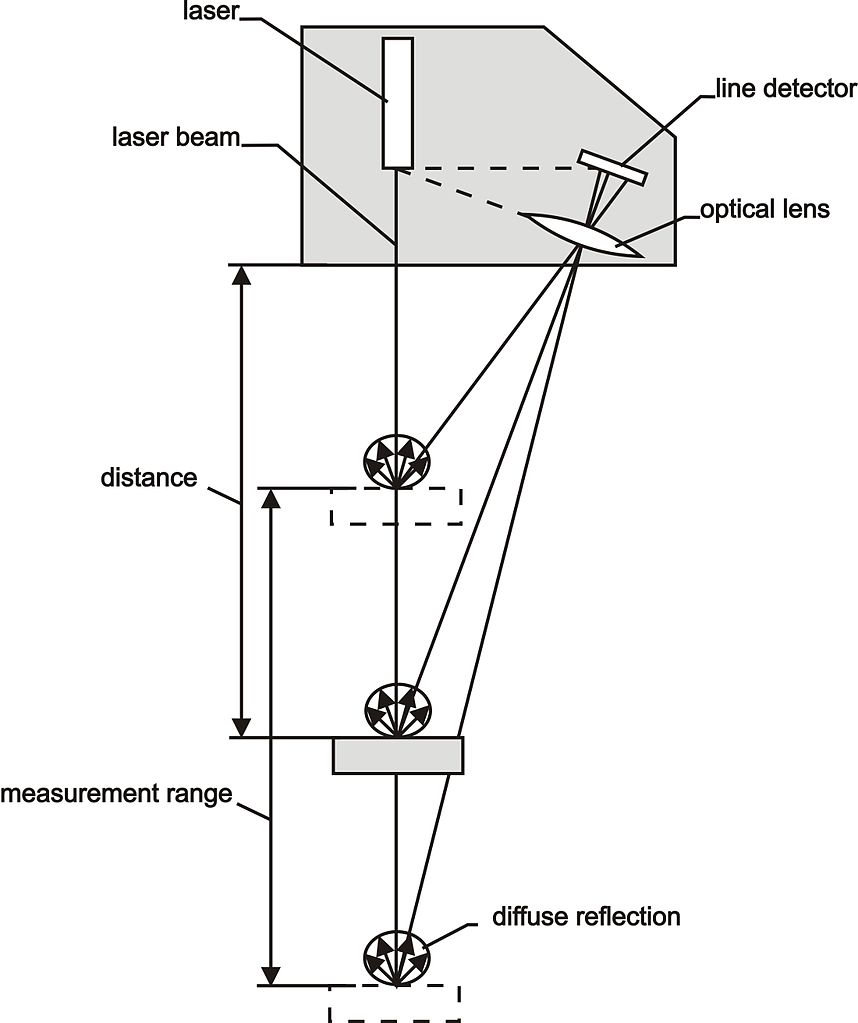
\includegraphics[width = 0.7\textwidth, frame]{./Bilder/triang.jpg}
\caption{Triangulation principle \cite{kwillms_english_2012}.}
\label{triang}
\end{figure}

The distance to this object is then calculated using the line detector. That is why it is called a position-based sensor.
The YDLIDAR X2 triangulation laser scanner rotates around its axis and scans the surrounding area with a scan angle of 360�. The angle resolution is 0.72�. The angle resolution is the angle difference between two consecutive scans.  These specifications are essential for the localization process and will be discussed in later chapters. In appendix \ref{chap:app1} the datasheet of the YDLIDAR X2 triangulation sensor is appended.


%
%
%--------------------------------------------------------------------
%
%
%
%
%--------------------------------------------------------------------
%
%
%
%
%--------------------------------------------------------------------
%
%
%--------------------------------------------------------------------
%
%Mustervorlage fuer eine Aufgabe
%
%--------------------------------------------------------------------
%
%Ueberschreiben der automatisch erzeugten Aufgabennummer
%Die folgende Aufgabennummer ergibt sich aus dem Stand des
%Z�hlers + 1
%\setcounter{chapter}{0}
%
\chapter{Methodology and Implementation}\label{chap:implementation}
%
%
%

This thesis consists of several components that run in unison to each other. Each component can be thought of as a building block to form a wall. To successfully build the wall each block must be carefully placed so that it effectively supports the next. In this chapter, the implementation and methodology of  each component will be explained.  

\section{Software architecture}
For a better understanding of the developed ROS software,  it's important to describe its architectural design and explain the connection between its different components. This section describes the overall ROS software architecture and the architecture of the implemented software.
 
In general, the architecture of any software which is based on ROS can be divided into two main layers. The first layer is the ROS computation graph. This computation graph contains nodes, topics, messages, and other components. The second layer is the ROS filesystem which contains all files and packages of the software.\citep{joseph_understanding_2015} A general example of the architecture design of a  software-based on ROS is shown in \ref{fig1}.  The components of each layer of the software are described and discussed in detail in the following sections. 

\begin{figure}[ht]
	\centering
	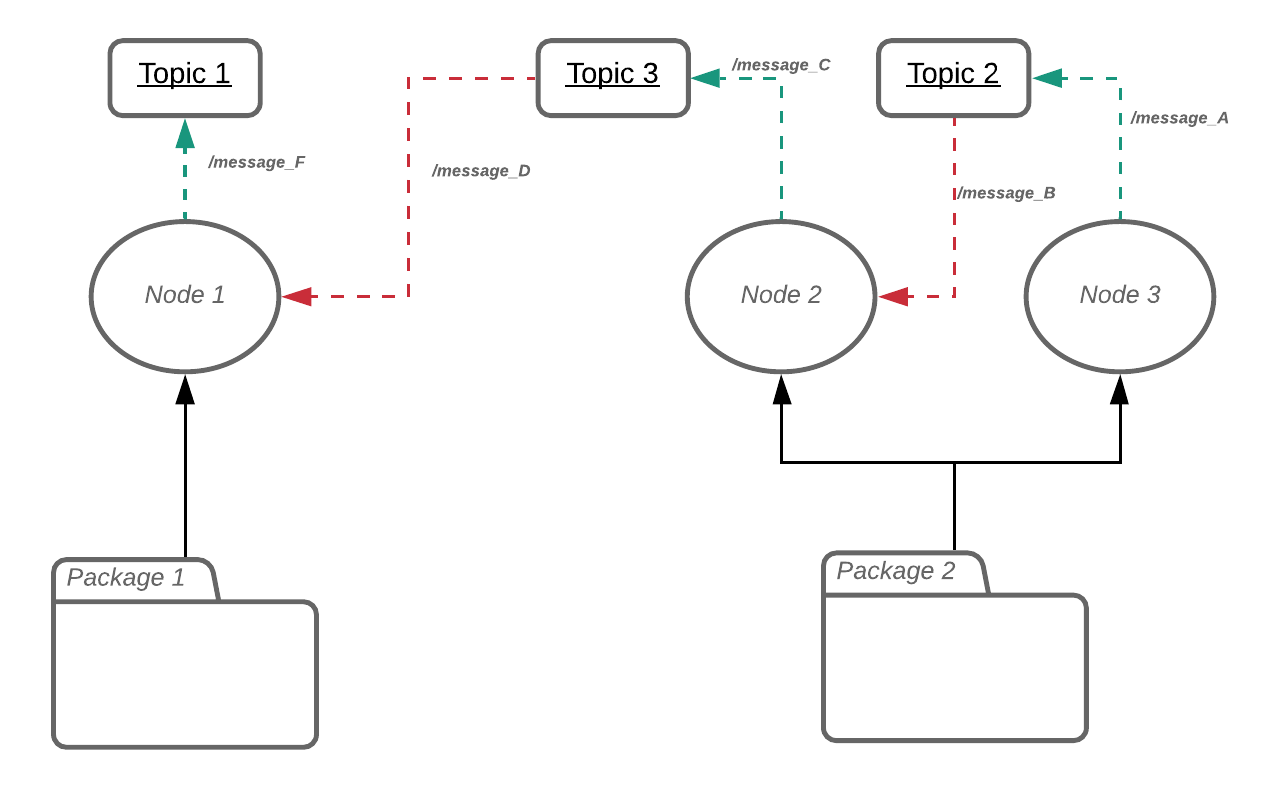
\includegraphics[width = 0.8\textwidth, frame]{./Bilder/UML_Architecture.png}			\caption{ROS architecture design}
	\label{fig1}
\end{figure}


\subsection{ROS filesystem:}


The top component of the filesystem is the catkin workspace which contains all used packages. Beneath the catkin workspace come the packages. The packages provide different tools and libraries, which could be used and configured to accomplish the desired functionalities. Each package contains messages, data types, services, and most importantly executable files and launch files \cite{joseph_understanding_2015}. The executable files, which are written either in C++ or in Python, are used to initialize ROS nodes. The launch files are used to configure and launch specific nodes. Since ROS is an open-source tool, all its packages can be found through the ROS Software Browser. During installation, there are some default packages that are recommended while downloading ROS. Other than this, all remaining packages must be downloaded or cloned individually from the Software Browser or alternatively be made from scratch. The following figure \ref{fig2} clearly demonstrates all the packages used in this project and the nodes that they include. 


\begin{figure}[ht]
	\centering
	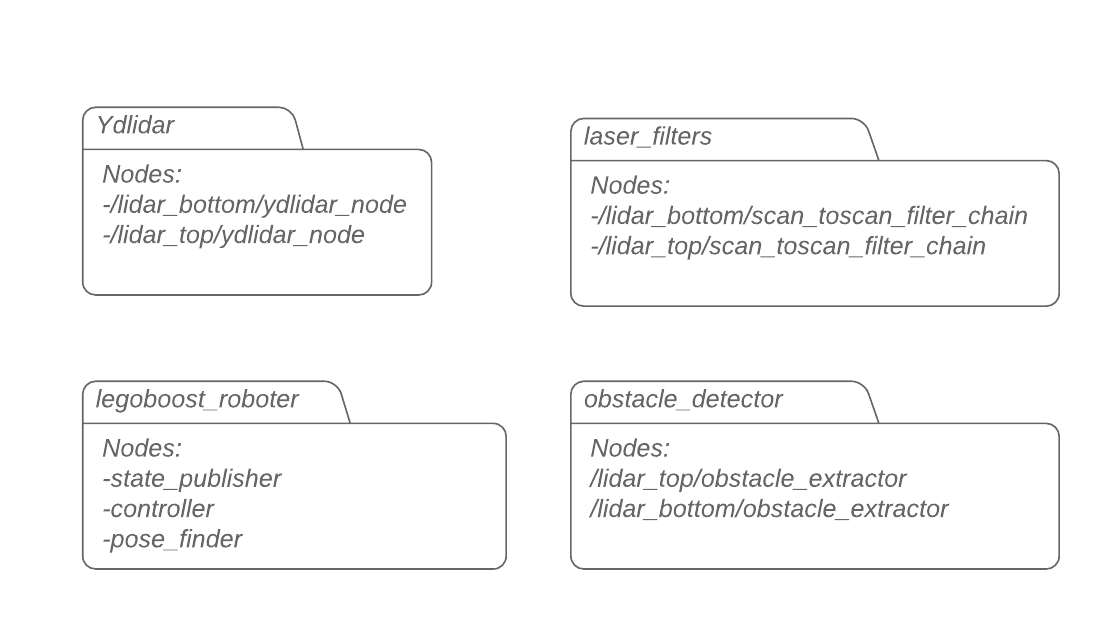
\includegraphics[width = 0.8\textwidth, frame]{./Bilder/UML_Packages.png}			\caption{ROS packages of the project}
	\label{fig2}
\end{figure}






Packages needed to be installed to support the default ROS packages are: 
\begin{enumerate}
\item \textbf{Ydlidar Package:} The first to be installed is the Ydlidar package, which supports the triangulation sensor package and is developed by Shenzhen EAI Technology Co. that produces. This has all the executable files that process the sensor data and publish it as a laserscan message to a topic. It also contains launch files for visualizing the sensor data in rviz. The nodes created in these packages are the /lidar-bottom/ydlidar-node contains all information about the bottom sensor while the /lidar-top/ydlidar-node contains all information about the top sensor. Further information about then nodes are discussed in the computation graph section \ref{subsec:computationGraph}.
\item  \textbf{The Laser-Filters Package:} this package is responsible for adjusting messages of type laserscan obtained from the triangulation sensor by using predefined filters so that it is suitable for later processing. Another option is to use pointCloud messages but this option is not required as the sensor publishes messages of type laserscan and not pointCloud. This package includes a node called scan-toscan-filter-chain, which is a pipeline of filters defined by the user \cite{foote_laser_filters_nodate}. It is useful for instances such as removing laser points off the wall in order to concentrate only on the robot laser scan data.
\item  \textbf{The Obstacle Detector Package:} This package is initially used for obstacle detection and tracking by using laserscan data from lidar sensors. However, in our case, this package is used to detect the robot. The node used in this package is called the obstacle-extractor node. This package also has a user-defined message type called "Obstacle" which includes the position of the obstacle in the XYZ plane. It also has nodes to visualize the obstacles in rviz. \cite{przybyla_tysikobstacle_detector_2020}
\item  \textbf{The Legoboost-Roboter Package:} Unlike the other packages, this one is made from scratch and contains all the information about the robot. This package consists of three main components; the controller, pose detector, and state publisher, each of which has a specific function. The state publisher consists of a node responsible for publishing the robots' frames and contains its URDF file. The pose detector is essentially a node that calculates the position and orientation of the robot using data collected from the obstacle collector. And lastly, the controller, which has a node that is responsible for the motion control of the robot.
\end{enumerate}





\subsection{ROS computation graph:}\label{subsec:computationGraph}



This section will go more in-depth on the computation graph layer for a better understanding of the software architecture. The computation graph is responsible for the connection between these components and the way the information is exchanged between these components. ROS node is one of the main components of the computation graph. It is responsible for computing a specific functionality or task.  ROS Nodes are connected together through topics or services. They could subscribe to topics to get the information from these topics and use this information to perform a specific task. They can also publish information to topics to post-process this information. Information that is exchanged between topics is called a message. Messages types can be either built-in, for example String or Bool, or can be defined by the user. \cite{joseph_learning_2018}. Figure \ref{fig3} shows the nodes used in this software and how they are interconnected. Any item within a square notions that this item is a topic, however an item within a circle relates to a node. This figure is generated by the rqt tool from ROS. This is a framework that is used for GUI purposes. 



\begin{figure}[ht]
	\centering
	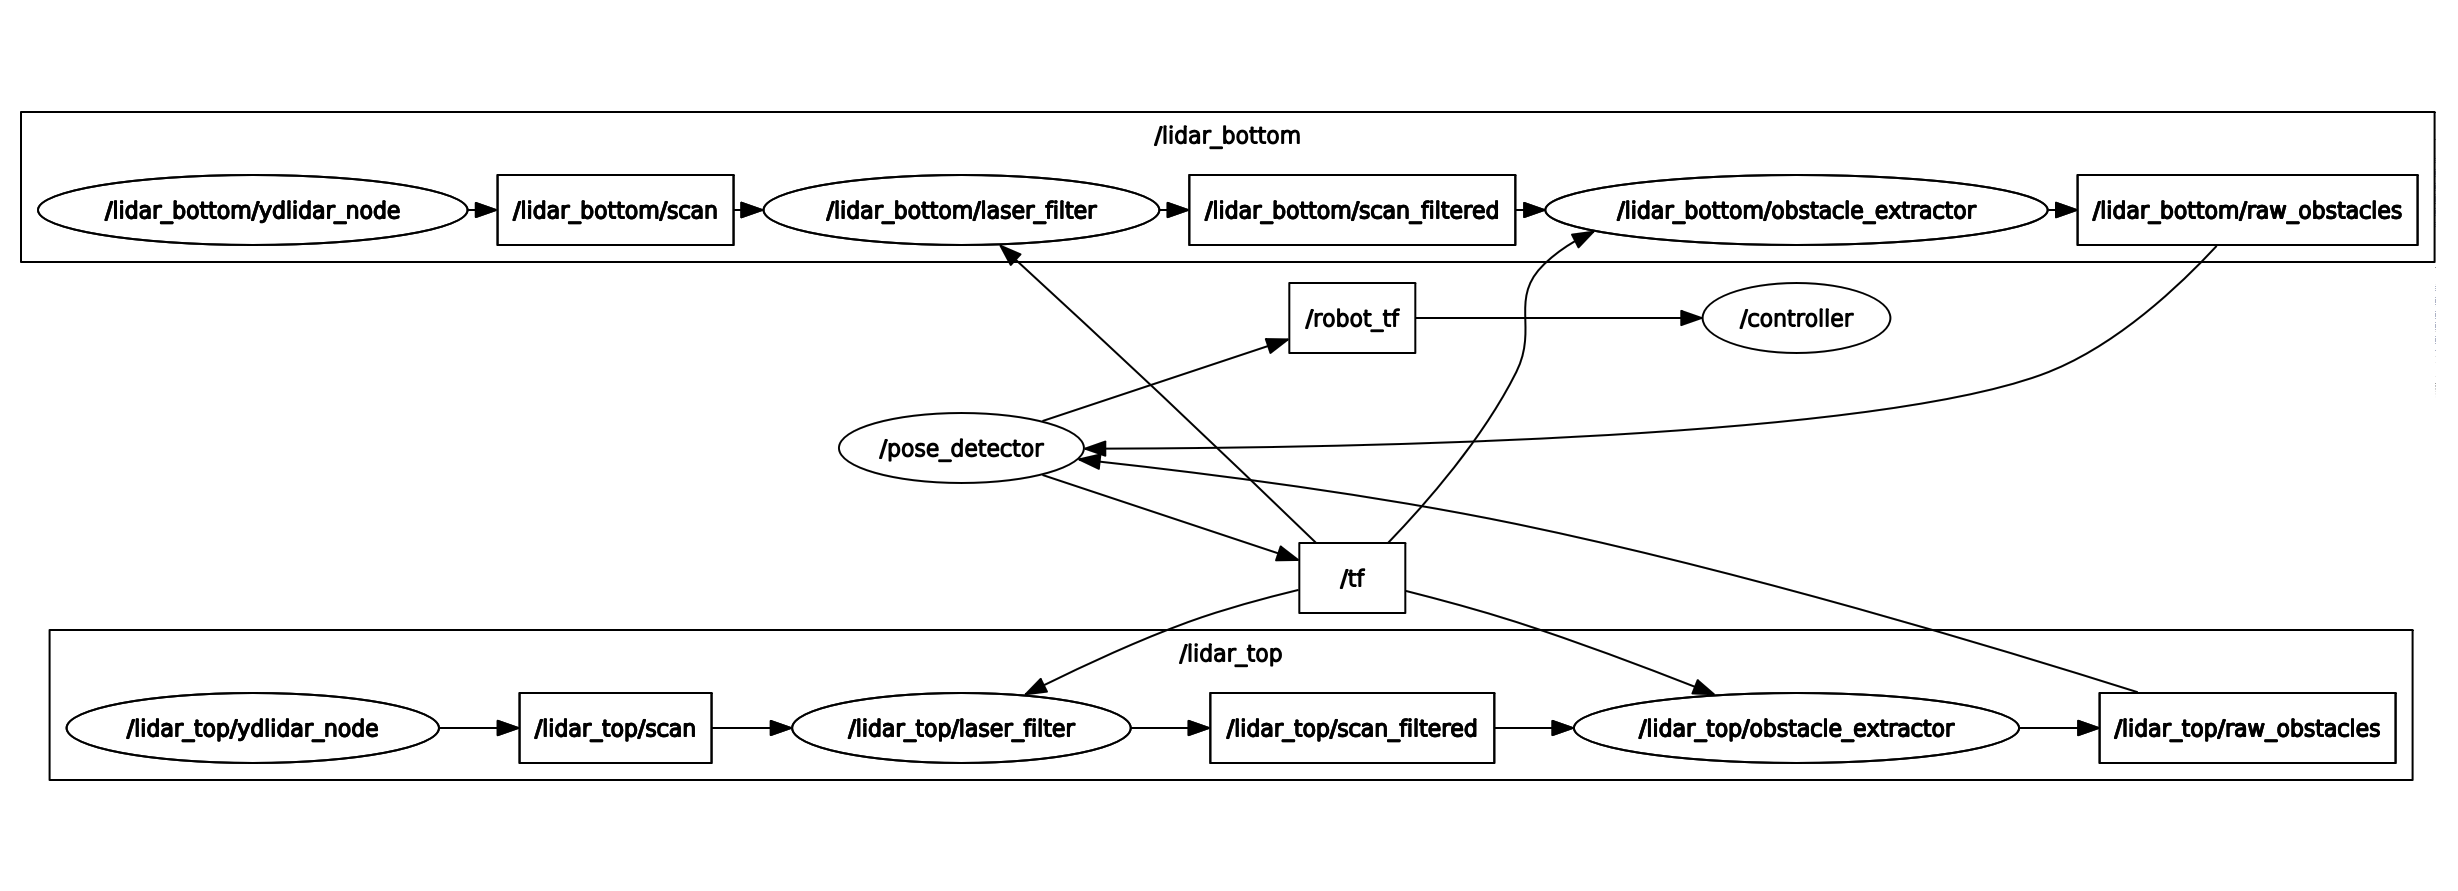
\includegraphics[width = 1.1\textwidth, frame]{./Bilder/rosgraph_nodes.png}			\caption{Relation between the nodes used in the project}
	\label{fig3}
\end{figure}


Since there are 2 sensors and the data of each sensor must be processed individually, it's important to launch separate nodes for each one. This can be done by using the attribute "ns" in the launch file. By using this attribute an instance of the node can be created in a user-defined namespace so that separate nodes are initiated. Figure \ref{fig3} shows these two namespaces, which are named "lidar\_bottom" and "lidar\_top".



As described in the previous figure, the nodes are:
\begin{enumerate}
\item \textbf{State-Publisher:} This node is responsible for publishing the jointstates and transformers of the robot.
\item \textbf{lidar\_bottom/ydlidar\_node and lidar\_top/ydlidar\_node:} These nodes publish messages of type laserscan to the topics "lidar\_bottom/scan" and "lidar\_top/scan" respectively. A LaserScan message in ROS sensor\_msgs package and it contains information about the sensor scans such as the ranges of each angle as well as the scan time and maximum and minimum range. \cite{noauthor_sensor_msgslaserscan_nodate}
\item \textbf{lidar\_bottom/scan\_filter and lidar\_top/scan\_filter} These nodes subscribe to the scan topics which are published from the ydlidar\_node and publish a filtered laserscan message to the topics "lidar\_bottom/filtered\_scan" and "lidar\_top/filtered\_scan". The scan\_filter nodes in each sensor use LaserScanBoxFilter, which exclude scan points that are outside a defined room\citep{foote_laser_filters_nodate}. The room is defined by two points in an XYZ-space. This is important to exclude the scan points of the room's walls. By doing this, only the scan points of the robot are going to be considered. Figure \ref{fig4} shows the plan view of the room, and the position of the sensors as well as the coordinates of the room. The XY coordinate of the sensors is (0,0), and the room's length as well as the room's width, is 1.6 meters. The sensor is placed 15 cm apart from the wall in both x and y directions. It's therefore concluded that  $P_{min}$ = (0.15,-0.15) and $P_{max}$ = (-1.45,1.45). 
\begin{figure}[ht]
	\centering
	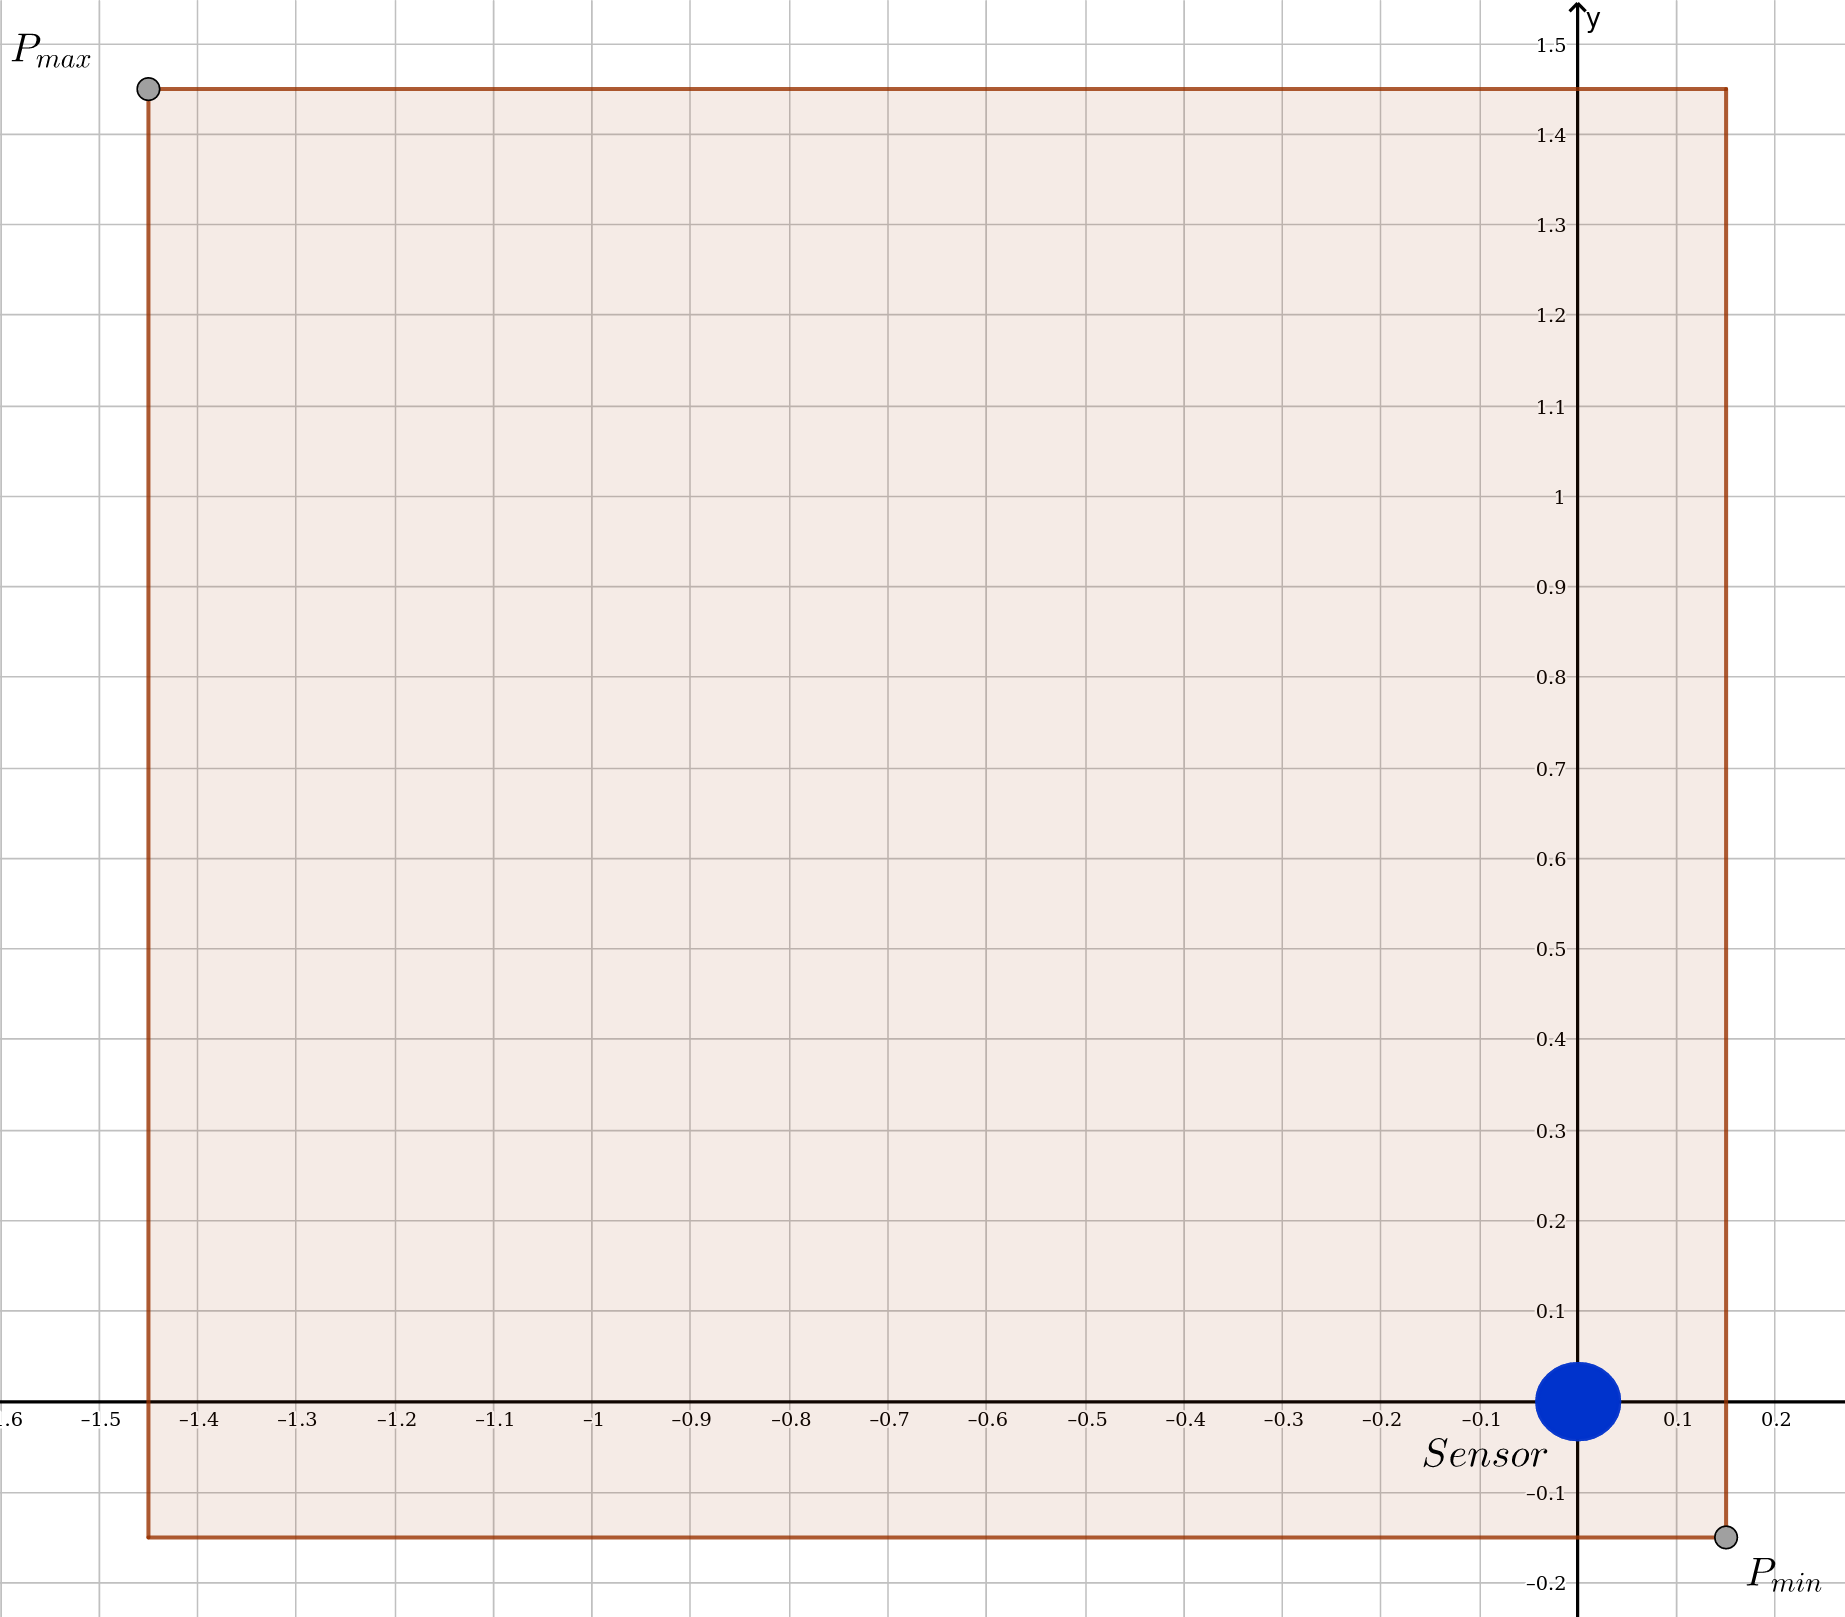
\includegraphics[width = 0.6\textwidth, frame]{./Bilder/room.png}			\caption{Plan view of the room}
	\label{fig4}
\end{figure}

\item \textbf{lidar\_top/obstacle\_extractor and lidar\_bottom/obstacle\_extractor:} subscribe to the scan\_filter topic of each sensor and  publish messages of type Obstacles to the topics "/lidar\_top/raw\_obstacles" and "/lidar\_bottom/raw\_obstacles."

\item \textbf{Pose\_Detector:} This node subscribes to the raw\_obstacle topic of each sensor and publishes the pose of the robot as a transformer message to the topic "robot\_tf". 

\item \textbf{Controller:} This node subscribes to the robot pose and publishes calculates the velocities of the left and right wheels. Then it sends velocity commands to the control unit. The implementation of obstacle extractor nodes as well as the pose\_detector node and controller node is discussed in further sections.
\end{enumerate}

\section{Robot architecture and visualization}

The design and visualization of the required system are two other building blocks that are essential for the successful completion of the project. This system consists of three main components, namely the robot, the sensors, and the room. In the first subsection, the specifications and requirements of each component in the system are explained in detail. Based on these requirements and specifications, the design of each component is going to be explained. \\
Visualizing various components of the system, including the robot, using visualization tools provided by the ROS are important for tracking results and monitoring the robot's motion.  In the second subsection, the visualization of the robot (system) in rviz is explained as well as the implementation of the robot's URDF.  

\subsection{Robot (System/Environment) design}

\textbf{System requirements:\\}
The first requirement of the system concerns the robot and sensor design. These two components must have a design that facilitates the localization process of the robot for the triangulation sensors to detect the position as well as the orientation of the robot. \\
The second requirement concerns the room design as it must be rectangular or square-shaped. Besides, the floor of the room must be a whiteboard and the sensors must be placed at a corner of the room. Lastly, the area of the room must be large enough for the robot to navigate within, yet not too large to ensure precise detection of the robot pose.

\textbf{System specifications:\\}
Some of the specifications of the robot are already known since they are closely tied to the Lego Move Hub specifications, referred to in Appendix X,  because it is the main control unit of the robot. However, other specifications must be included that are based on the requirements discussed above.
\begin{enumerate}
\item Communication Protocol:
Move Hub uses a Bluetooth Low Energy (BLE) processor for the communication between the control unit and the PC. The Bluetooth communication is based on GATT protocol.
\item Steering system:
Since Move Hub has two separated motors, each controlled individually, then the steering system of the robot is differentially steered. This steering system is nonholonomic.
\item Robot design:
The design of the robot and is related to the first requirement mentioned previously. After several trials with different designs, a specific design was achieved as follows:
\begin{itemize}
\item The robot has two cylinders with the same radius. One of these cylinders is placed at the front and the other at the back of the robot. 
\item The cylinders are placed in different XZ planes. 
\item  The cylinders are wrapped with non-reflective papers, so that the laser doesn't reflect and lead to data loss. 
\end{itemize}
The following figure \ref{fig:fig5} shows the design of the robot. The design is made by Mecabricks.com which is a web service to design models using Lego bricks. 
\begin{figure}[ht]
\begin{subfigure}[c]{0.5\textwidth}
  \centering
  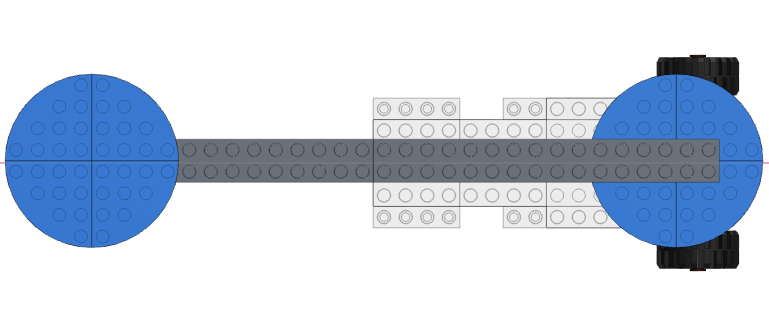
\includegraphics[width=1\linewidth]{./Bilder/Robot_Top.png}
  \caption{Plan view}
  \label{fig5:sfig1}
\end{subfigure}%
\begin{subfigure}[c]{0.5\textwidth}
  \centering
  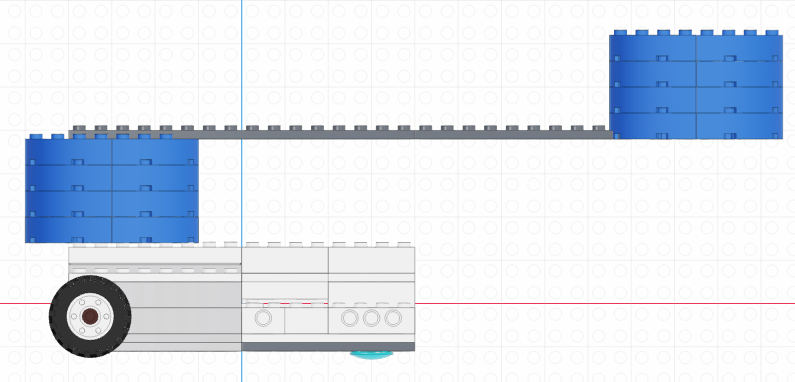
\includegraphics[width=0.8\linewidth]{./Bilder/Robot_Side.png}
  \caption{Side view}
  \label{fig5:sfig2}
\end{subfigure}
\caption{Plan and side view of the robot.}
\label{fig:fig5}
\end{figure}
\item Sensors design:
The system has 2 sensors each determine a different cylinder. The sensors are placed on each other with the same orientation, so that the x and y-axis of both sensors are identical. The sensor which is placed on top is on the same plane as the cylinder which is placed on top. The same applies to the other sensor. 
\item Room design:
The fifth specification is the design of the room and is related to the second requirement mentioned in the requirements above. To design the room, it's important to consider two aspects. The first one is  the sensor's specifications, which are discussed in section \ref{sec:lidar}. The second aspect is the ability of the obstacle detector algorithm, which is used to detect the cylinders. By considering these aspects, the maximum area of the room can be determined as follows.\\
The angle increment of the sensor is 0.72 $\frac{degree}{step}$. To detect obstacles using the obstacle detector algorithm at least 5 laser beams of the object must be valid. The first and the last beam values are actually the tangents of the cylinder. The minimum valid angle between those tangents indicates the maximum length between the sensor and the obstacle. This angle is calculated as follows: 
\begin{equation}
\theta_{min} = i*R_{min}
\end{equation}
where \hspace{15mm} $i$  =  angle increment\\ 
	  \hspace*{25mm} $R_{min}$  =  minimum number of ranges

The challenge now is to find this maximum length using this angle. This can be done by basic geometry rules. The following figure \ref{fig6} shows circle B which has a radius. The tangents of the circle are connected to the same point $A$. Theta is the angle between the tangents. 

\begin{figure}[ht]
	\centering
	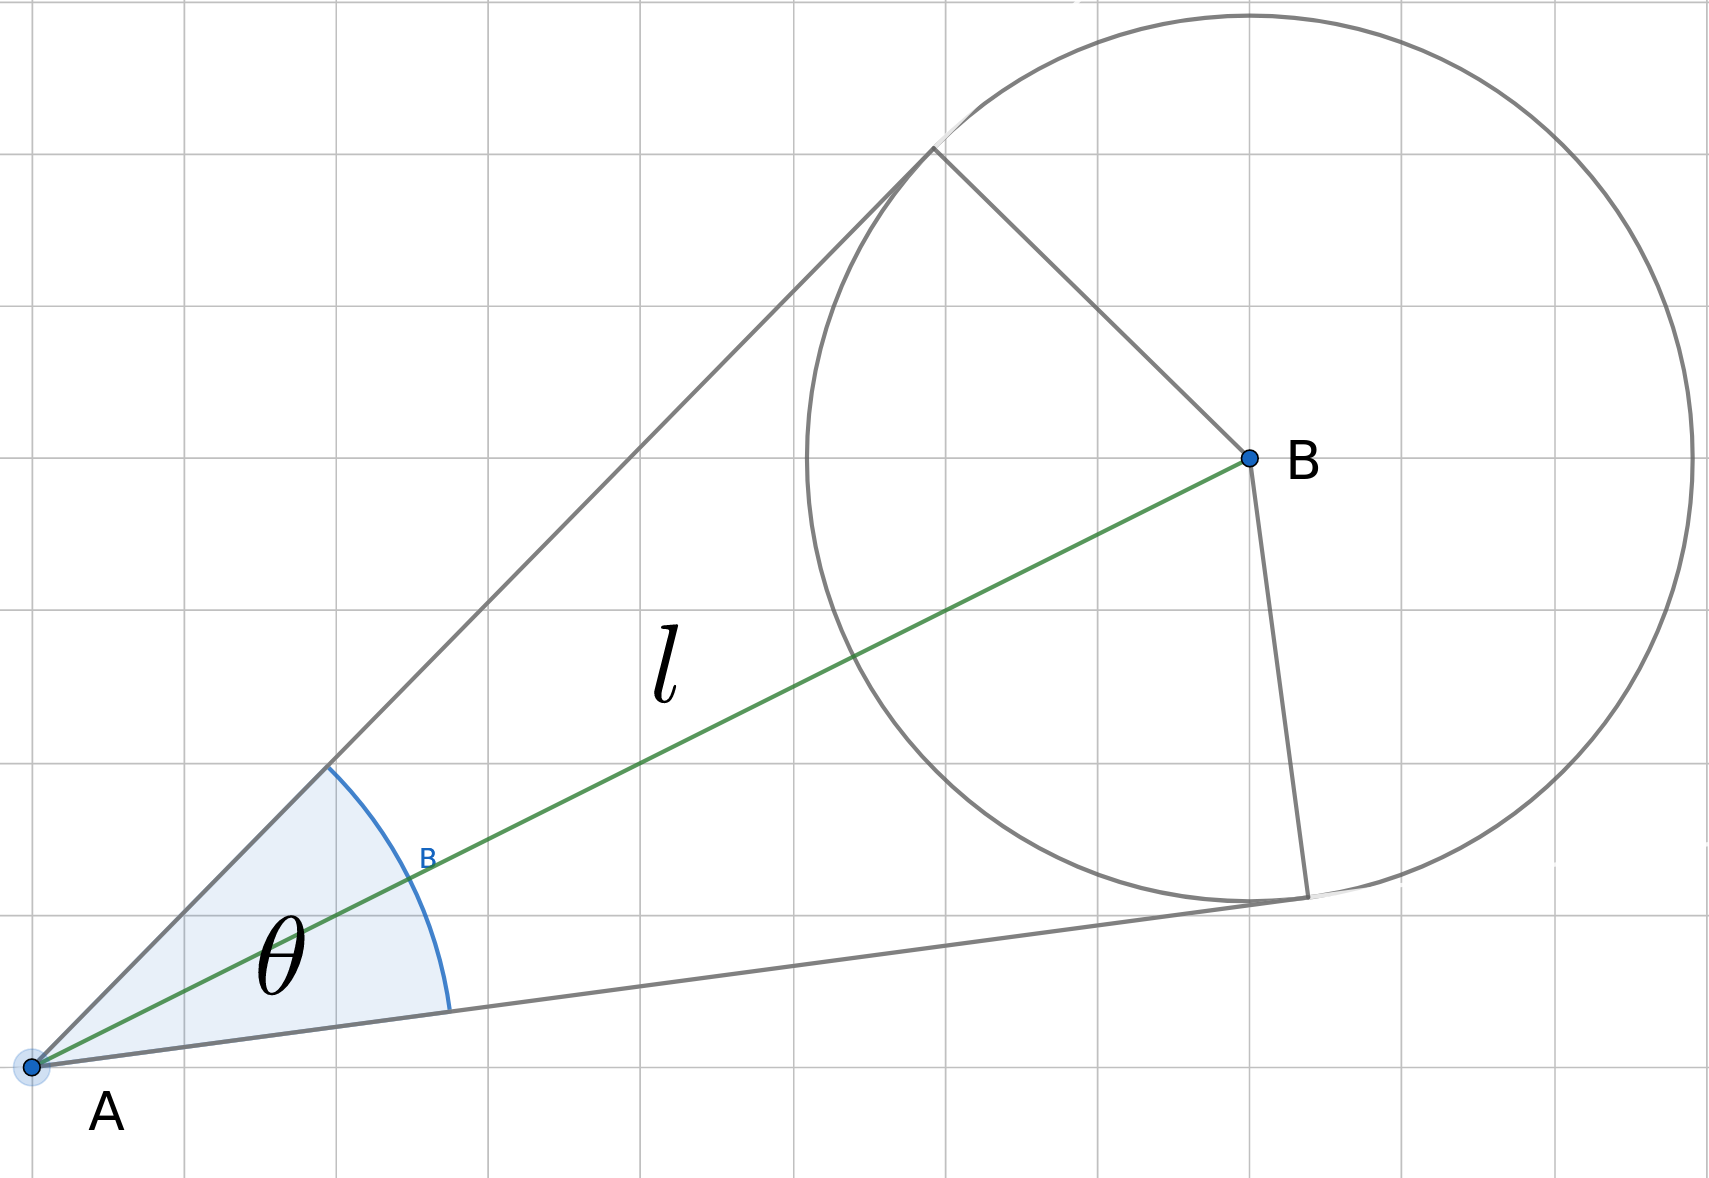
\includegraphics[width = 0.6\textwidth, frame]{./Bilder/geogebra.png}			\caption{The Relation of the length between external point and center of a circle and the angle between circle tangents to this point}
	\label{fig6}
\end{figure}


The length $l$ can be calculated as follows:
\begin{equation} \label{eq1}
l= \frac{r}{sin(\frac{\theta}{2})}
\end{equation}

by substituting theta from equation (1) in equation (2):
\begin{equation} \label{eq2}
l_{max} = \frac{r}{sin(\frac{i*R_{min}}{2})}
\end{equation}
where \hspace{15mm} $i = 0.72 \hspace{1mm}\frac{degree}{step}$\\ 
	  \hspace*{25mm} $R_{min} \geq 5$ steps
	  
From this equation, the room dimensions could be specified. By using cylinders with radius $r$ = 62 mm. Then $l_{max}$ = 2.5 m. The maximum distance in the room is the diagonal. The length of each side of the room could be calculated by using the following equation:
\begin{equation} \label{eq3}
a = \frac{l_{max}}{\sqrt{2}} = 1,768 m
\end{equation}
Yet it's important to consider the error analysis of the previously discussed method. Since the Lidar sensor has a relative error of 1.5\% for any distance between 0.5 m and 6m, and since there are 2 different sensors, then FRAGE(Error calculation)
\end{enumerate}

\subsection{Robot/Model Visualization}
Visualizing the robot and the other components of the system using visualization tools that are provided by ROS is important for watching the results and monitoring the robot motion. The visualization tool used in ROS applications is called RViz, which is a GUI used to subscribe to topics and visualize the data in these topics. RViz contains specific display types for specific message types. For example, LaserScan display type displays the data from a sensor\_msg::LaserScan message. However new display types could be added by using user-defined plugins. For example an obstacle display type is added to Rviz using a user-defined plugin. Another display type is the Robot Model, which represents the robot pose depending on its URDF. The URDF is an XML file which describes the joints and the links of the robot and the relation between them.\cite{noauthor_urdfxmljoint_nodate}




 That being said, the next step is to write the URDF file of the LegoBoost robot.  The URDF of LegoBoost robot is simple. It consists of 4 links and 3 joints. The first joint is the base joint, which connects between two links, namely the base footprint which is the parent link, and the base link which is the child link. The base footprint demonstrates the position of the robot at the ground level. The base link is the position of the center of mass of the robot. It's placed above the base footprint\cite{noauthor_rep_nodate}. These two links are connected through a fixed joint named base joint. The base joint is fixed since it doesn't have any degree of freedom. The second joint is the right wheel joint, which connects the base link to the right wheel link. The last joint is the left wheel joint, which connects between the base link and the left wheel link. The hierarchy of the URDF  and the connection between the different links and joints is shown in figure \ref{fig7}. This figure is generated by urdf\_to\_graphviz tool.

\begin{figure}[ht]
	\centering
	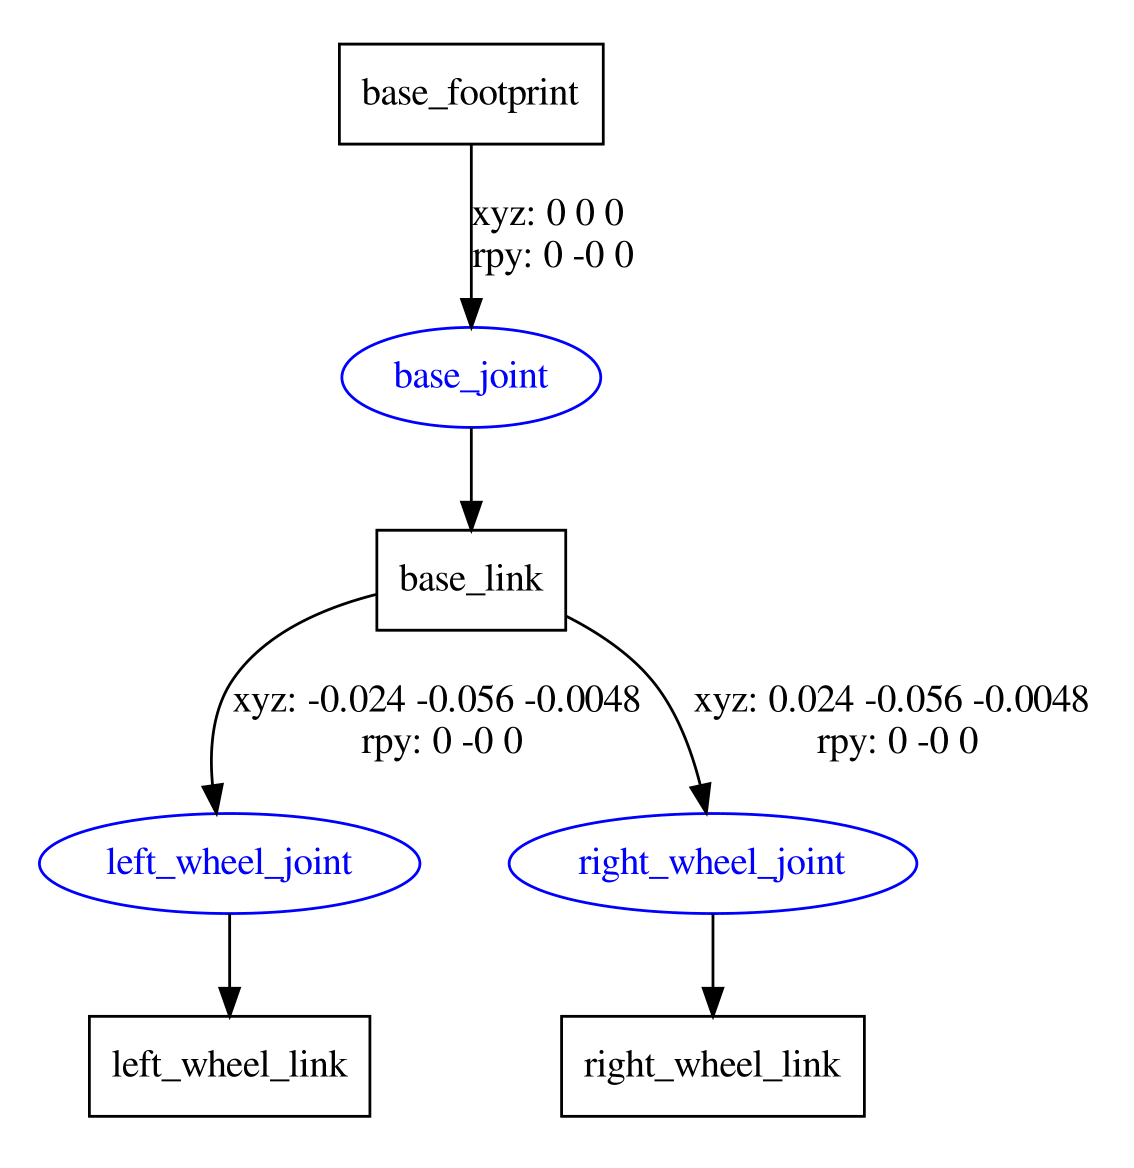
\includegraphics[width = 0.6\textwidth, frame]{./Bilder/legoboost_robot.png}			\caption{Graphical demonstration of LegoBoost URDF}
	\label{fig7}
\end{figure}


Each link in the URDF file can contain visual properties. The visual properties could be used for a better visualization of the robot. The geometry of both right and left wheel links are implemented in the URDF as cylinders with the same radius of the robot's wheels. The base link geometry is implemented as a box with the same dimensions of the robot.\\
After implementing the URDF file, the next step is to set up the Rviz tool and add all the required display types, which are:
\begin{itemize}
\item Robot model: This displays the URDF of the robot.
\item LaserScan: This displays the scan data of the sensors. A LaserScan display type is added for each sensor.
\item Obstacles: This displays the cylinders on the robot. An obstacle is added to each cylinder. Each cylinder is colored differently, namely red for the top cylinder and blue for the bottom cylinder. 
\item TF: This displays the TF transform hierarchy of the model. 
\end{itemize} 
The final visualization of the whole model in RViz is shown in figure \ref{fig8}. The frames of the sensors as well as the robot are demonstrated. The red and white points demonstrate the laserscans of the sensors and the red cylinder shows the front cylinder of the robot. The cylinder at the back is not shown in this figure for simplicity and clearer vision.
\begin{figure}[ht]
	\centering
	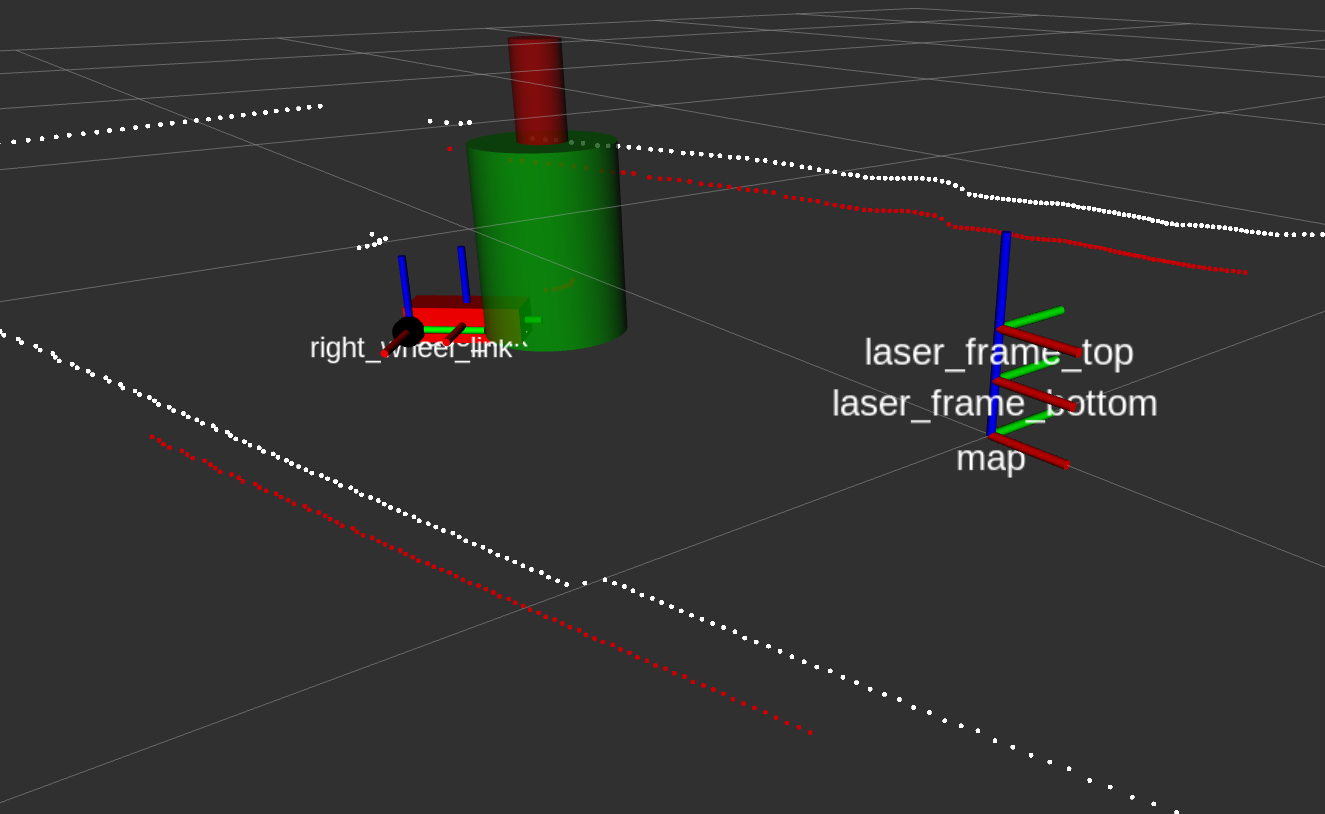
\includegraphics[width = 0.9\textwidth, frame]{./Bilder/rviz_screenshot.png}
	\caption{The model visualization in RViz}
	\label{fig8}
\end{figure}

\section{Robot localization}
Robot localization is another essential building block in the project and the core of the thesis.   Under robot localization two things must be considered. First, is localizing the position of the robot, and second, localizing the orientation of the robot. Both the orientation and the position represent the pose of the robot. Localization in mobile robots context is usually performed by using SLAM algorithms, where a lidar sensor or a camera is integrated in the robot to scan the surrounding environment and the SLAM algorithms are used to build a map of this environment and localize the pose of the robot depending on this map and other inputs like the odometry of the robot \cite{ros_book}. In contrast to the SLAM algorithms, the method used in this thesis is however different, since the sensors are not integrated in the robot but fixed in a specific place in the room. From the perspective of the sensor, the surrounding environment is still, and only the robot is moving. In this section, the used methods, which have been used for the robot localization are going to be discussed. Firstly, localization using the obstacle detector approach is discussed. Then the localization using image processing is discussed. At last, the localization using laser scan matcher approach is discussed.

\subsection{Circular object detection approach}   %8 pages
%1)introduction and explain how the algorithm work   1page
%2)how did I implement the approach to detect the robot pose 6pages
%	2.1 Idea explanation (Geometry)
%	2.2 Code explanation
%3)how accurate is the detection 1 page
%4) conclusion 1 page


Obstacles detection algorithms are essential in robot navigation. Such algorithms are used for example during navigation to avoid obstacles. The obstacle detection algorithm developed in \cite{obstacle_detector} is used for detecting circle-shaped obstacles by using circles geometric properties and the polynomial regression of laser scan data. The main reason for choosing this algorithm is its fascinating efficiency and speed. According to the applied tests mentioned in \cite{circle} the accuracy rate of the circles' detection is 92.53\% and the average executing time is 16 $ms$ per frame which is around $50 Hz$. This is more than twice the publishing rate of the sensor, which is $20 Hz$.  The main idea of using this algorithm is to detect the cylinders, that are placed on the robot. By detecting the exact position of these cylinders, the pose of the robot could be calculated. 



\subsection{Image Processing approach} %4 pages
%1)introduction and explain how the algorithm work
%2)how did I implement the approach to detect the robot pose
%	2.1 Idea explanation (Geometry)
%	2.2 Code explanation
%3) Difficulties, and why didn't I continue working on this approach


\subsection{Laser scan matcher approach} %4 pages
%1)introduction and explain how the algorithm work
%2)how to implement the laser scan matcher. which data are used as inputs and %what is the output of the algorithm (Computational graph)
%3) Difficulties, and why didn't I continue working on this approach



%--------------------------------------------------------------------
%
%Mustervorlage fuer eine Aufgabe
%
%--------------------------------------------------------------------
%
%Ueberschreiben der automatisch erzeugten Aufgabennummer
%Die folgende Aufgabennummer ergibt sich aus dem Stand des
%Z�hlers + 1
%\setcounter{chapter}{0}
%
\chapter{Results and Future Work}\label{chap:results}
%
%
%
In the previous chapters, different components of the project have been discussed. After setting up the ROS system on the computer, the laser scanner was put into operation, and the robot was built. Then several localization algorithms were used and tested. Lastly, the control was implemented, and the whole system was integrated all together. As explained before, the robot must follow a pre-defined line. In this chapter, the results of the control algorithm will be discussed. Finally, improvements and future work will be discussed.

\section{Control Results}
 

As explained before, the robot follows a given line, which can be described with equation \ref{eq14}. In order to test the control algorithm, three different equations will be used. These equations are:

\begin{equation}\label{eq20}
y + x = 0 
\end{equation}
\begin{equation}\label{eq21}
y - 0.5 = 0 
\end{equation}
\begin{equation}\label{eq22}
x + 0.5 = 0 
\end{equation}

Each equation corresponds to a different line. Equation \ref{eq22} corresponds to a straight line that is parallel to the Y-Axis. This line will be labeled as Path A. Path B is a straight line that is parallel to the X-Axis, which corresponds to equation \ref{eq21}. Lastly, Path C, which is a sloped line that corresponds to equation \ref{eq20}. For each equation, different initial poses will be tested. The poses are noted as following $(x,y,\theta)$, where $x$ and $y$ correspond to the position of the robot, and $\theta$ corresponds to the orientation of the robot. The different pathes are plotted in runtime using MatplotLib library.\\

\textbf{Path A:}\\
As displayed in figure \ref{fig:fig15}, two different initial poses have been considered. The first initial pose is $(-0,1.15,180�)$. The second initial pose is $(-0,1.15,180�)$. In both cases, the robot successfully controlled its motion to follow the given line.

\begin{figure}[ht]
\begin{subfigure}[c]{1\textwidth}
  \centering
  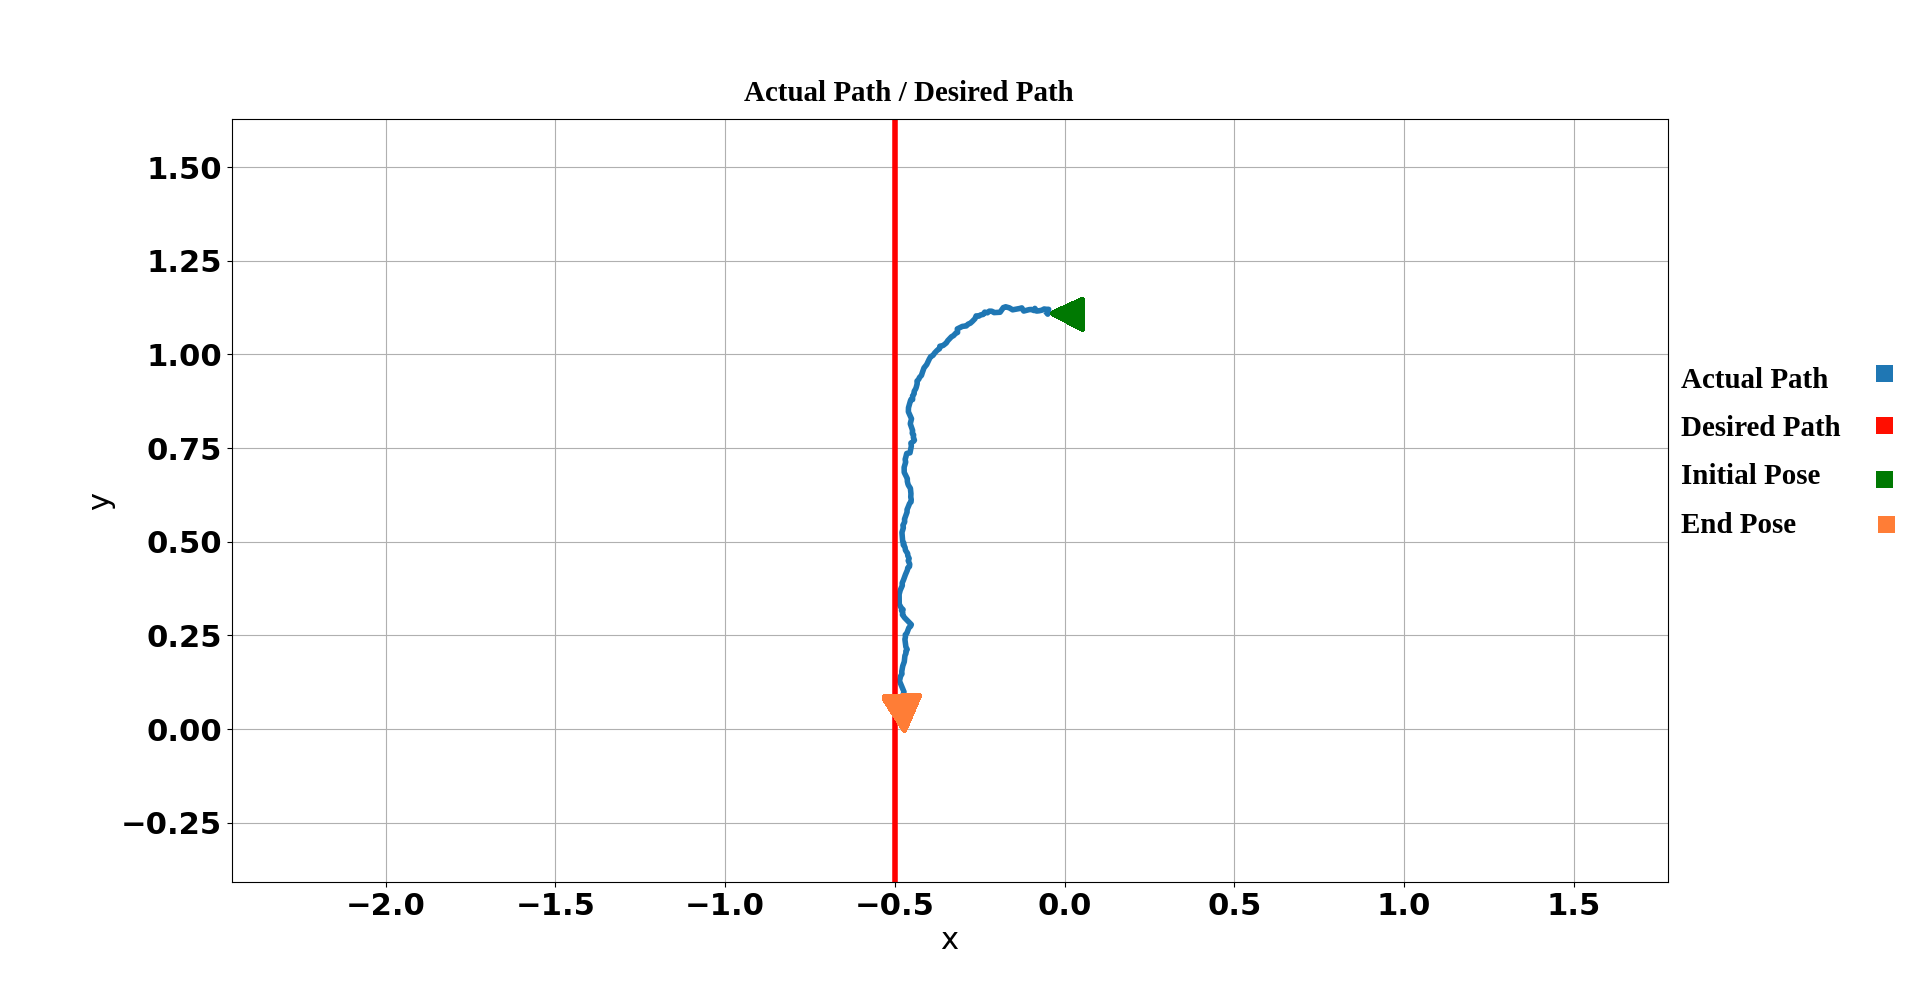
\includegraphics[width=1\linewidth]{./Bilder/Figure_1A.png}
  \caption{First initial pose}
  \label{fig15:sfig1}
\end{subfigure}%

\hspace*{\fill}%          % empty line absolutely necessary!
\begin{subfigure}[c]{1\textwidth}
  \centering
  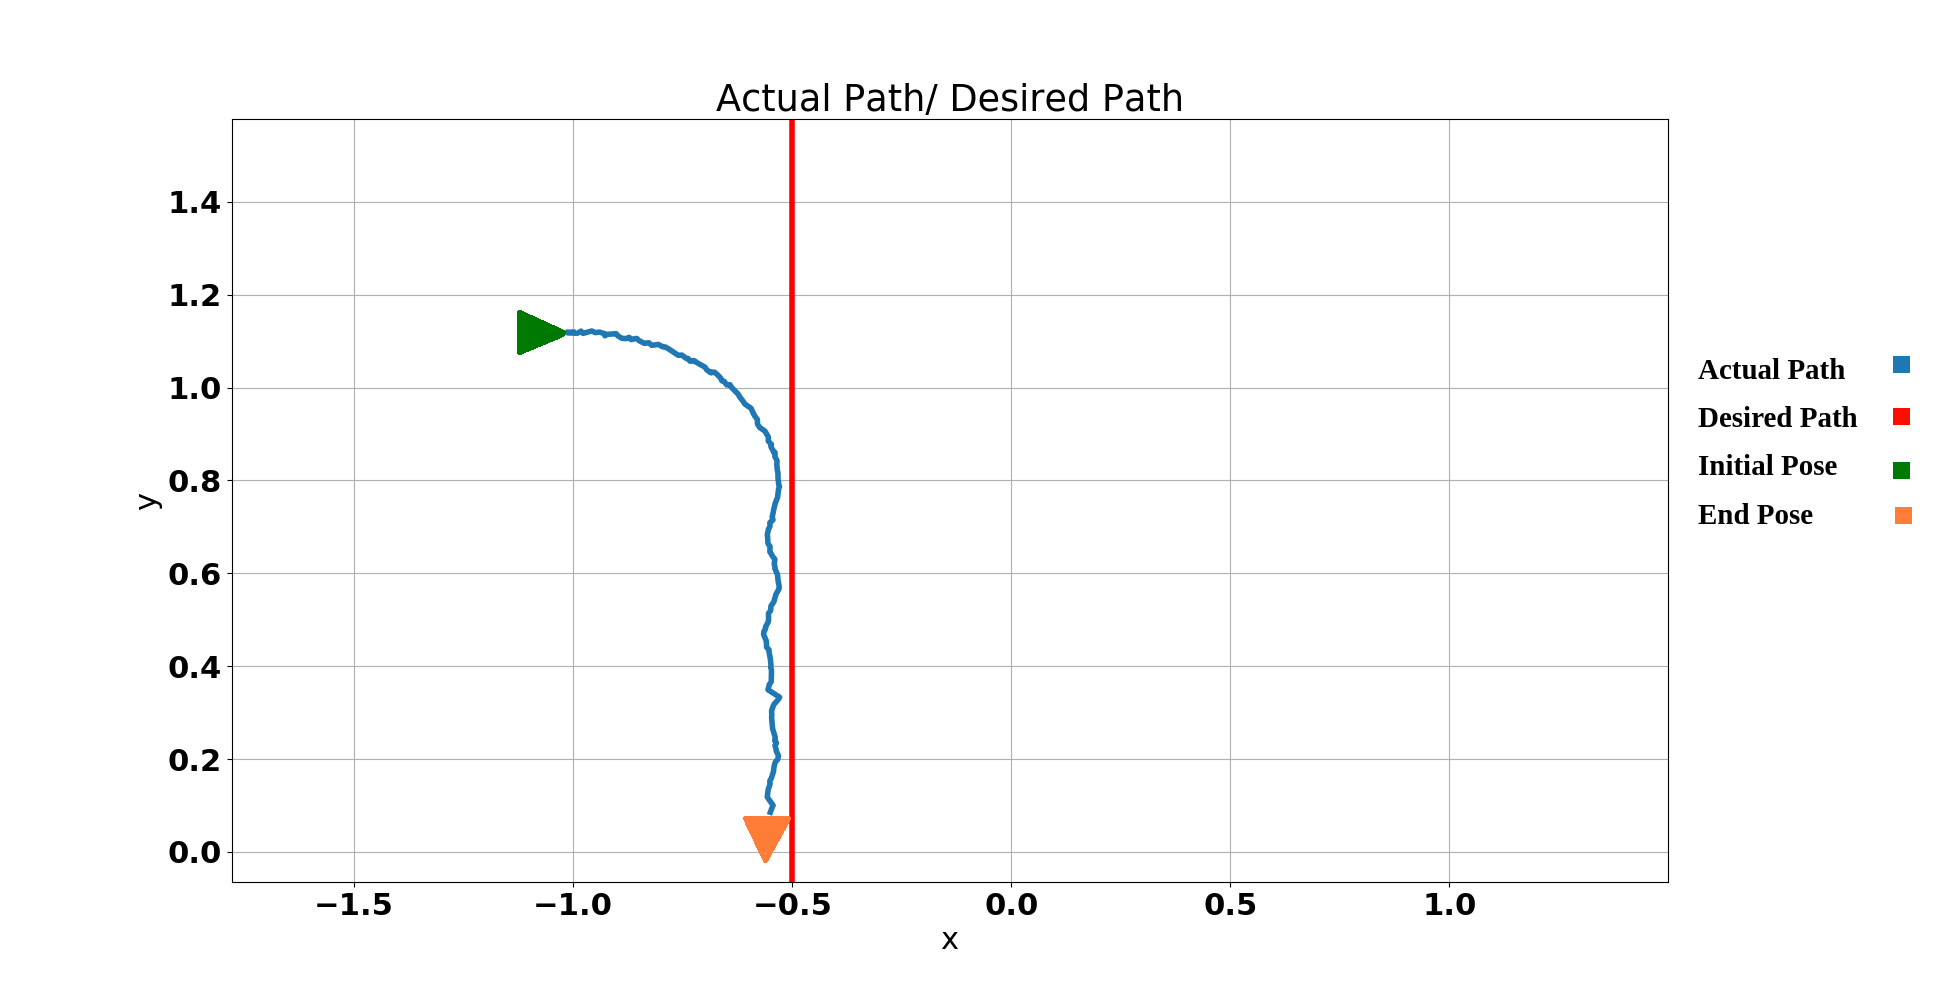
\includegraphics[width=1\linewidth]{./Bilder/Figure_1B.png}
  \caption{Second initial pose} 
  \label{fig15:sfig2}
\end{subfigure}
\caption{Robot motion control: Path A.}
\label{fig:fig15}
\end{figure}
 
\textbf{Path B:}\\
The same as in Path A, two different initial poses have been considered. The first initial pose is $(-0.21,0.05,90�)$. The second initial pose is $(-0.05,1.1,315�)$. In both cases, the robot successfully controlled its motion to follow the given line. The motion of the robot in both cases is displayed in figure \ref{fig:fig16}


\begin{figure}[ht]
\begin{subfigure}[c]{1\textwidth}
  \centering
  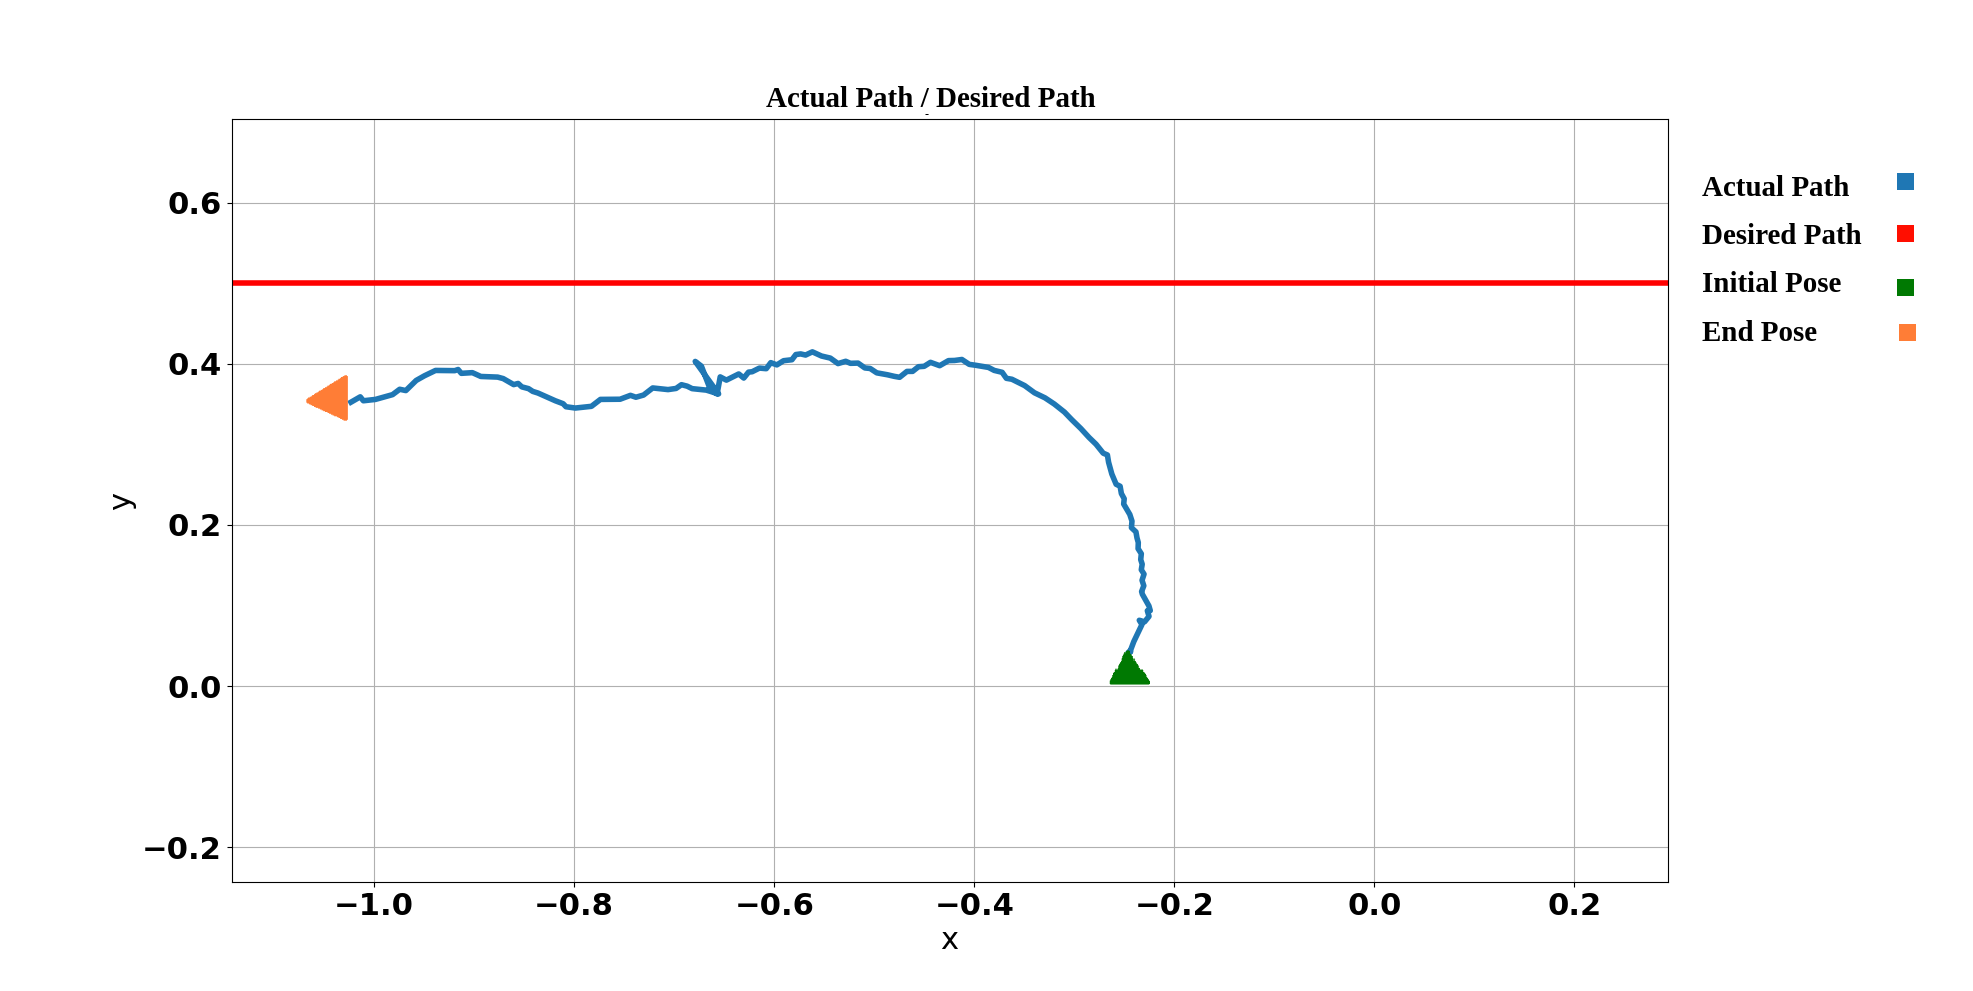
\includegraphics[width=1\linewidth]{./Bilder/Figure_2A.png}
  \caption{First initial pose}
  \label{fig16:sfig1}
\end{subfigure}%

\hspace*{\fill}%          % empty line absolutely necessary!

\begin{subfigure}[c]{1\textwidth}
  \centering
  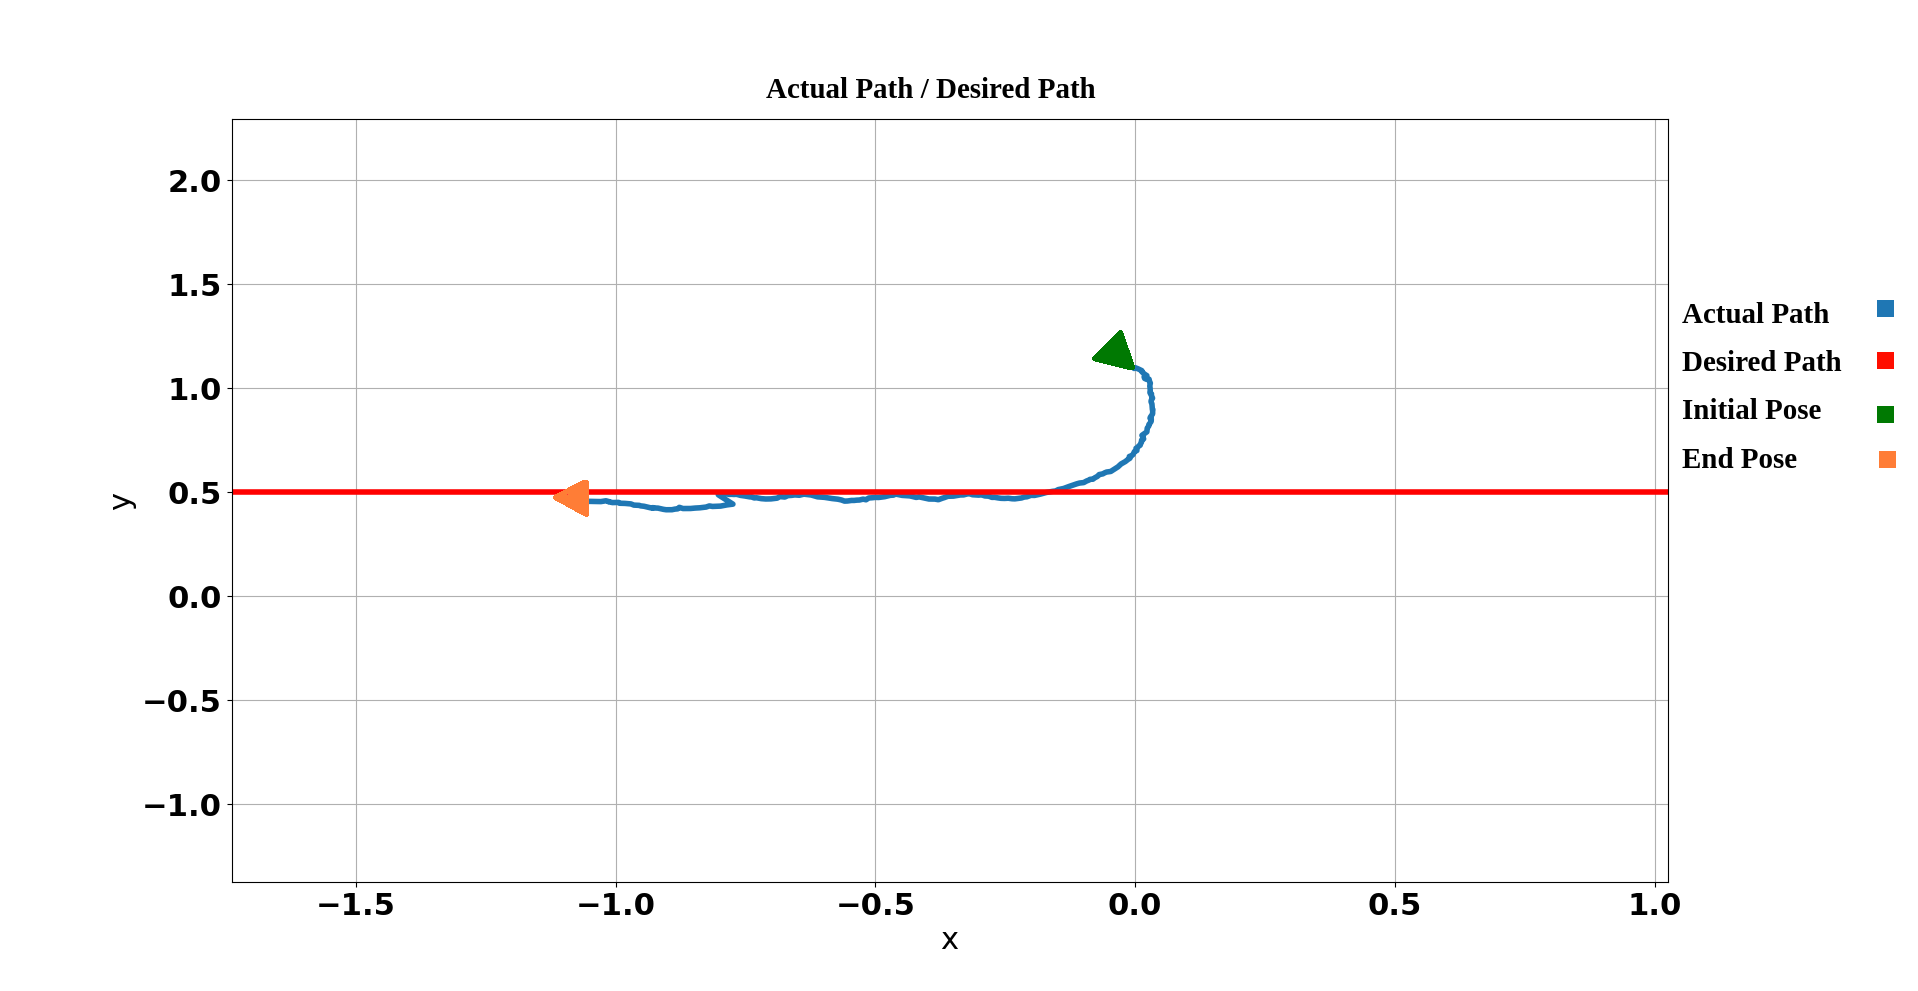
\includegraphics[width=1\linewidth]{./Bilder/Figure_2B.png}
  \caption{Second initial pose} 
  \label{fig16:sfig2}
\end{subfigure}
\caption{Robot motion control: Path B.}
\label{fig:fig16}
\end{figure}
 

\textbf{Path C:}\\
As displayed in \ref{fig17}, the initial pose of the robot is $(-0.25,0,90�)$. The robot follows the given line.
\begin{figure}[ht]
	\centering
	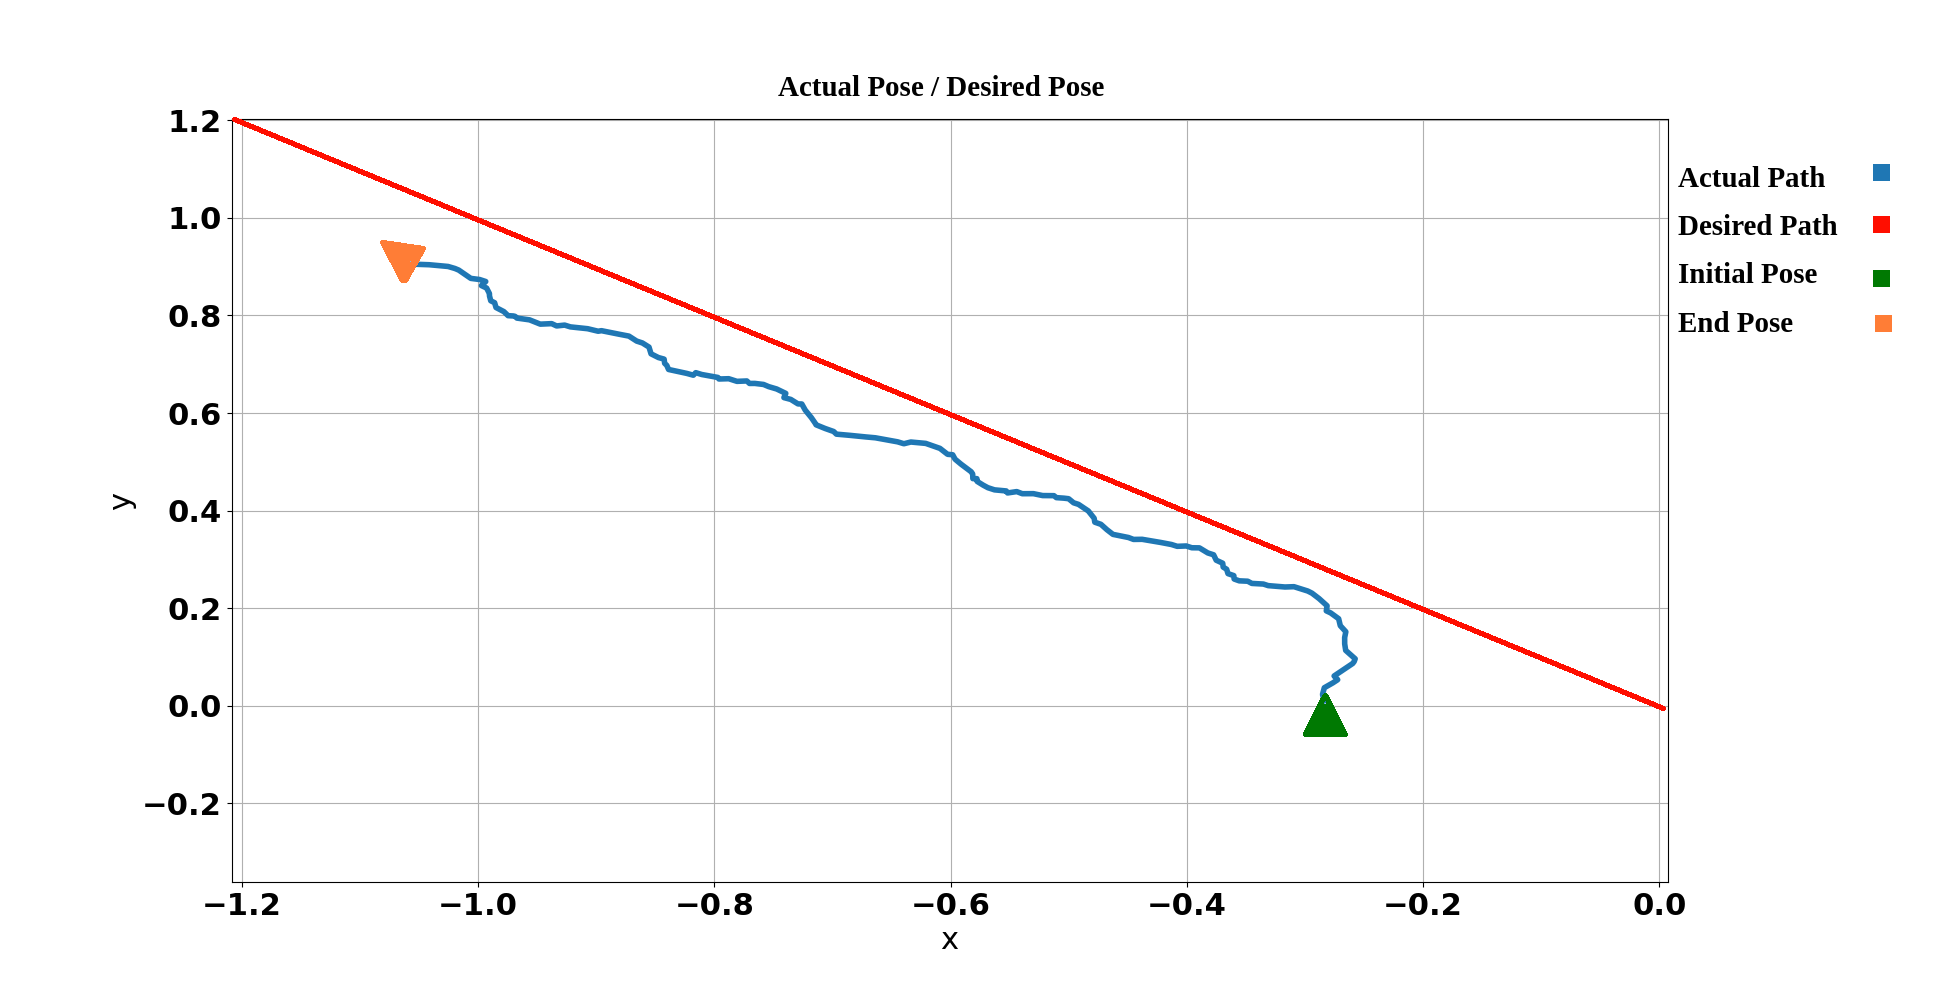
\includegraphics[width = 1\textwidth]{./Bilder/Figure_3A.png}
	\caption{Robot motion control: Path C}
	\label{fig17}
\end{figure}\\


As displayed in the previous figures, the robot was able to follow the pre-defined lines as expected. However, since two different proportional controllers are used, there is an offset to the given path. This offset occurs due to the inaccuracy of the proportional controller. Another problem that can be observed is the oscillations of the robot motion after the distance is minimized. This problem can be solved by adding a hysteresis.\\

Although the performance of the control algorithm was not ideal, this approach provides several advantages. The most important advantage is the extensibility of the software. In other words, other nodes and components can be added easily to the software to improve the results or even to add new features. Another advantage of this approach is the reusability of the nodes. The control algorithm node, for example, can be used to any other robot. The presented results show the feasibility.
An optimization of the control system will improve the behaviour considerably, but unfortunately could not be tackled in the time frame of this work.


\section{Future Work} 

As explained before, since this project based on ROS, other components can be added and integrated into the software. Thus, many different applications and ideas can be added. The next step is to add other control algorithms, i.e., to let the robot follow a trajectory or to make it move to a specific pose. Many of these control algorithms are explained in \cite{corke_robotics_2017}. Moreover, the whole system can be simulated using Gazebo. Gazebo is a simulation tool used in the field of robotics to simulate robots.
Furthermore, the system can also be extended to contain more than one robot at the same time. 
%--------------------------------------------------------------------
%
%Mustervorlage fuer eine Aufgabe
%
%--------------------------------------------------------------------
%
%Ueberschreiben der automatisch erzeugten Aufgabennummer
%Die folgende Aufgabennummer ergibt sich aus dem Stand des
%Z�hlers + 1
%\setcounter{chapter}{0}
%
\chapter{Summary}\label{chap:summary}
%
%
%
In conclusion, this thesis presents a new approach for mobile robot localization and navigation. This approach is different than other used approaches as it uses only a laser scanner. The laser scanner is fixed in the room. The idea behind that is to scan the surrounding area and detect the pose of the robot based on the scan information. The software used in this thesis was developed under ROS, which has different advantages as code extensibility and reusability. The project contains separate modules, namely the motion control, the localization, the laser scanner and the robot. In order to localize the robot, three different methods have been tested. After comparing the three methods, the circular object detection method has been used due to its efficiency and accuracy. Finally, a control algorithm was used to let the robot move along a pre-defined line. In order to test the controller, different pre-defined paths were given as input to the controller. Given that this was only a preliminary attempt to use this approach, it is important to improve the controller algorithm to achieve better performance. Furthermore, it is recommended to simulate the whole system using simulation tools like Gazebo, which is usually used for robotics applications developed under ROS.


%--------------------------------------------------------------------
%
%Mustervorlage fuer eine Aufgabe
%
%--------------------------------------------------------------------
%
%Ueberschreiben der automatisch erzeugten Aufgabennummer
%Die folgende Aufgabennummer ergibt sich aus dem Stand des
%Z�hlers + 1
%\setcounter{chapter}{0}
%
%
%
%
\begin{appendices}
\chapter{YDLIDAR X2 Datasheet}\label{chap:app1}

\begin{figure}[ht]
\centering
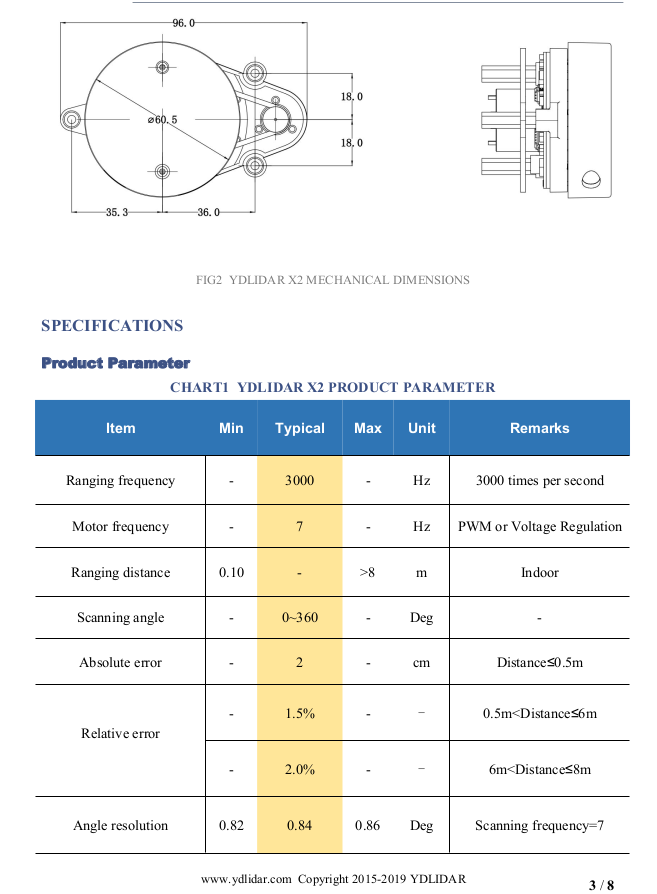
\includegraphics[width = 0.8\textwidth, frame]{./Bilder/sensorappendix.png}
\caption{YDLIDAR X2 triangulation laser scanner. \textcopyright YDLIDAR All rights reserved }
\label{ydlidar}
\end{figure}

\chapter{Directory Structure}\label{chap:app2}

\begin{figure}[ht]
\centering
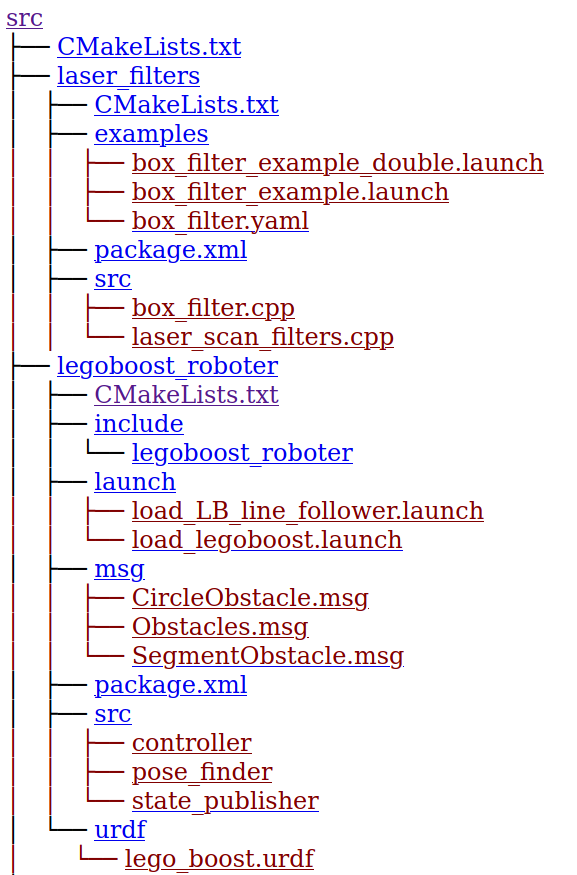
\includegraphics[width = 0.7\textwidth]{./Bilder/tree_app1.png}

\end{figure}

\begin{figure}[ht]
\centering
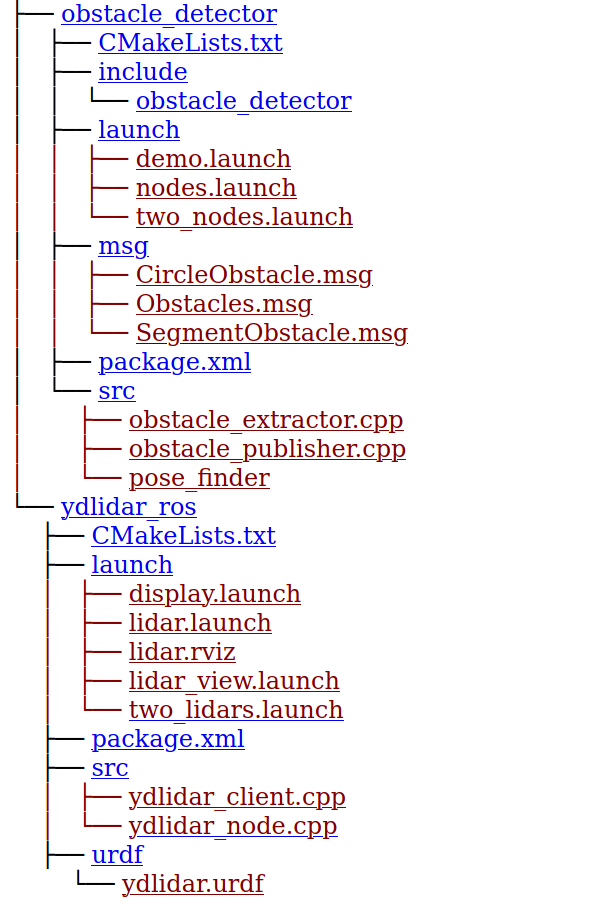
\includegraphics[width = 0.7\textwidth]{./Bilder/tree_app2.png}
\end{figure}
\end{appendices}


%
%und m�glicherweise noch andere Aufgaben
%

%
%Literaturverzeichnis bei Bedarf
%

\bibliographystyle{unsrt}
\bibliography{Exported_Items}
%
%
\end{document}

